\documentclass[12pt, a4paper]{report}
\usepackage{style}


\title{Data Bases II \\ \textit{Theory}}
\author{Christian Rossi}
\date{Academic Year 2023-2024}

\begin{document}

\maketitle

\newpage

\begin{abstract}
    The course aims to prepare software designers on the effective development of database applications. 
    
    First, the course presents the fundamental features of current database architectures, with a specific emphasis on the concept of transaction and its realization in centralized 
    and distributed systems. 
    
    Then, the course illustrates the main directions in the evolution of database systems, presenting approaches that go beyond the relational model, like active databases, object 
    systems and XML data management solutions.
\end{abstract}

\newpage

\tableofcontents

\newpage

\chapter{Introduction}
    \section{Data Base Management System}
    \begin{definition}
        A \emph{Data Base Management System} is a software product capable of managing data collections that are: 
        \begin{itemize}
            \item Large: much larger than the central memory available on the computers that run the software. 
            \item Persistent: with a lifetime which is independent of single executions of the programs that access them. 
            \item Shared: used by several applications at a time. 
            \item Reliable: ensuring tolerance to hardware and software failures. 
            \item Data ownership respectful: by disciplining and controlling accesses. 
        \end{itemize}
    \end{definition}
    \begin{chronology}[5]{1990}{2020}{\textwidth}
        \event{1992}{SQL '92}
        \event{1999}{SQL '99}
        \event{2001}{Ranking in databases}
        \event{2003}{XML-related features}
        \event{2005}{NoSQL}
        \event{2006}{X-Query}
        \event{2009}{JPA final release}
        \event{2011}{Temporal databases}
        \event{2016}{JSON}
    \end{chronology}

    \section{Transactions}
    \begin{definition}
        A \emph{transaction} is an elementary, atomic unit of work performed by an application. Each transaction is conceptually encapsulated within two commands:
        \begin{itemize}
            \item Begin transaction.
            \item End transaction.
        \end{itemize}
    \end{definition}
    Within a transaction, one of the commands below is executed to signal the end of the transaction: commit or rollback. 
    \begin{definition}
        The \emph{On-Line Transaction Processing} (OLTP) is a system that supports the execution of transactions on behalf of concurrent applications. 
    \end{definition}
    The application can run many transactions. So, the transactions are part of the application and not vice-versa. The transactions follow the ACID property: 
    \begin{enumerate}
        \item Atomicity: a transaction is an indivisible unit of execution. This means that all the operations in the transaction are executed or none is executed. The time in which 
            commit is executed marks the instant in which the transaction ends successfully: an error before should cause the rollback and an error after should not alter the 
            transaction. The rollback of the work performed can be caused by a rollback statement or by the DBMS. In case of a rollback, the work performed must be undone, bringing 
            the database to the state it had before the start of the transaction. It is the application's responsibility to decide whether an aborted transaction must be redone or not. 
        \item Consistency: A transaction must satisfy the database integrity constraints, that is if the initial state $S_0$ is consistent then the final state $S_f$ is also 
            consistent. This is not necessarily true for the intermediate states $S_i$. 
        \item Isolation: the execution of a transaction must be independent of the concurrent execution of other transactions. 
        \item Durability: the effect of a transaction that has successfully committed will last forever, independently of any system fault. 
    \end{enumerate}
    \begin{table}[H]
        \centering
        \begin{tabular}{c|c|c}
        \textbf{Property} & \textbf{Actions}       & \textbf{Architectural element} \\ \hline
        Atomicity         & Abort-rollback-restart & Query Manager                  \\
        Consistency       & Integrity checking     & Integrity Control System       \\
        Isolation         & Concurrency control    & Concurrency Control System     \\
        Durability        & Recovery management    & Reliability Manager           
        \end{tabular}
    \end{table}
    \begin{figure}[H]
        \centering
        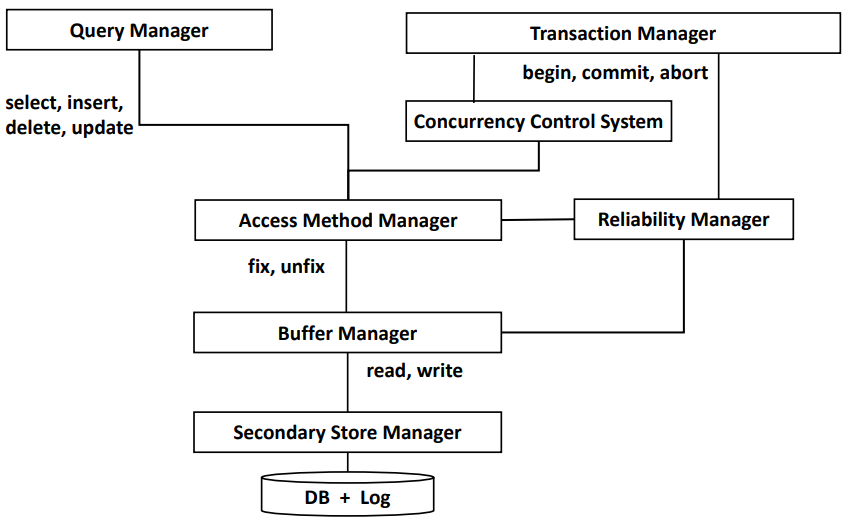
\includegraphics[width=0.75\linewidth]{images/architecture.png}
        \caption{Architecture of a Data Base Management System}
    \end{figure}

\newpage

\chapter{Concurrency}
    \section{Introduction}
    A DBMS usually needs to manage multiple applications. A unit of measurement used to evaluate the DBMS workload is the number of transaction per second ($tps$) handled by it. 
    To have an efficient usage of the database the DBMS needs to be able to handle concurrency while avoiding the insurgence of anomalies. 
    The concurrency control system schedules the order of the various transactions. 
    
    \section{Anomalies in concurrent transactions}
    The anomalies caused by uncorrect scheduling are: 
    \begin{itemize}
        \item Lost update: an update is applied from a state that ignores a preceding update, which is lost.
            \begin{table}[H]
                \centering
                \begin{tabular}{c|c}
                \textbf{Transaction $t_1$}    & \textbf{Transaction $t_2$} \\ \hline
                $r_1(x)$                      &                            \\
                $x=x+1$                       &                            \\
                                              & $r_2(x)$                   \\
                                              & $x=x+1$                    \\
                                              & $w_2(x)$                   \\
                                              & commit                     \\
                $w_1(x)$                      &                            \\
                commit                        &                           
                \end{tabular}
            \end{table}
        \item Dirty read: an uncommitted value is used to update the data. 
            \begin{table}[H]
                \centering
                \begin{tabular}{c|c}
                \textbf{Transaction $t_1$} & \textbf{Transaction $t_2$} \\ \hline
                $r_1(x)$                   &                            \\
                $x=x+1$                    &                            \\
                $w_1(x)$                   &                            \\
                                        & $r_2(x)$                   \\
                                        & commit                     \\
                abort                      &                           
                \end{tabular}
            \end{table}
        \item Non-repeatable read: someone else updates a previously read value.
            \begin{table}[H]
                \centering
                \begin{tabular}{c|c}
                \textbf{Transaction $t_1$}  & \textbf{Transaction $t_2$} \\ \hline
                $r_1(x)$                    &                            \\
                                            & $r_2(x)$                   \\
                                            & $x=x+1$                    \\
                                            & $w_2(x)$                   \\
                                            & commit                     \\
                $r_1(x)$                    &                            \\
                commit                      & \multicolumn{1}{l}{}      
                \end{tabular}
            \end{table}
        \item Phantom update: someone else updates data that contributes to a previously valid constraint. 
            \begin{table}[H]
                \centering
                \begin{tabular}{c|c}
                \textbf{Transaction $t_1$} & \textbf{Transaction $t_2$} \\ \hline
                $r_1(x)$                   &                            \\
                                           & $r_2(y)$                   \\
                $r_1(y)$                   &                            \\
                                           & $y=y-100$                  \\
                                           & $r_2(z)$                   \\
                                           & $z=z+100$                  \\
                                           & $w_2(y)$                   \\
                                           & $w_2(z)$                   \\
                                           & commit                     \\
                $r_1(z)$                   &                            \\
                $s=x+y+z$                  &                            \\
                commit                     &                           
                \end{tabular}
            \end{table}
        \item Phantom insert: someone else inserts data that contributes to a previously read datum.
    \end{itemize}

    \section{Concurrency theory}
    \begin{definition}
        A \emph{model} is an abstraction of a system, object or process, which purposely disregards details to simplify the investigation of relevant properties. 
    \end{definition}
    Concurrency theory builds upon a model of transaction and concurrency control principles that help understanding the real systems. Real systems exploit implementation level 
    mechanisms which help achieve some desirable properties postulated by the theory. 
    \begin{definition}
        An \emph{operation} consist in a reading or in a writing of a specific datum by a specific transaction. 

        A \emph{schedule} is a sequence of operations performed by concurrent transactions that respects the order of operations of each transaction. 
    \end{definition}
    The transactions can be: serial, interleaved or nested. The number of serial schedules for $n$ transaction is equal to: 
    \[N_S=n!\]
    While the total number of distinct schedules given the number of transaction $n$ is equal to: 
    \[N_D=\dfrac{\left( \sum_{i=1}^nk_i \right)!}{\prod_{i=1}^n \left( k_i! \right)}\]
    \begin{example}
        Given two transaction $T_1$ and $T_2$ we have six possible different schedules, where only two are serial:
        \begin{enumerate}
            \item $r_1(x) w_1(x) r_2(z) w2(z)$
            \item $r_2(z) w_2(z) r_1(x) w_1(x)$
            \item $r_1(x) r_2(z) w_1(x) w_2(z)$
            \item $r_2(z) r_1(x) w_2(z) w_1(x)$
            \item $r_1(x) r_2(z) w_2(z) w_1(x)$
            \item $r_2(z) r_1(x) w_1(x) w_2(z)$
        \end{enumerate}
        The first two are serial, the third and the fourth are nested, and the last two interleaved.
    \end{example}
    The concurrency control has to reject all the schedules that causes anomalies. 
    \begin{definition}
        The \emph{scheduler} is a component that accepts or rejects operations requested by the transactions. 

        The \emph{serial schedule} is a schedule in which the actions of each transaction occur in a contiguous sequence.
    \end{definition}
    A serializable schedule leaves the database in the same state as some serial schedule of the same transactions, so it is correct. To introduce other classes we have to initially
    make two assumptions: 
    \begin{itemize}
        \item The transactions are observed a posteriori. 
        \item Commit-projection: consider only the committed transactions. 
    \end{itemize}

    \section{View-serializability}
    \begin{definition}
        $r_i(x)$ \emph{reads-from} $w_j(x)$ when  $w_j(x)$  precedes  $r_i(x)$ and there is no  $w_k(x)$ in $S$ between  $r_i(x)$  and  $w_j(x)$. 
        
        $w_i(x)$ in a schedule $S$ is a \emph{final write} if it is the last write on $x$ that occurs in $S$. 


        Two schedules are said to be \emph{view-equivalent} ($S_i \approx_V S_j$) if they have:
        \begin{enumerate}
            \item The same operations. 
            \item The same reads-from relationships.
            \item The same final writes. 
        \end{enumerate}
    \end{definition}

    A schedule is view-serializable (VSR) if it is view-equivalent to a serial schedule of the same transactions. The value written by $w_j(x)$ could be uncommitted when $r_i(x)$ 
    reads it, but we are sure that it will be committed (commit-projection hypotesis).
    \begin{example}
        The following schedules are given:
        \begin{itemize}
            \item $S_1: w_0(x) r_2(x) r_1(x) w_2(x) w_2(z)$
            \item $S_2: w_0(x) r_1(x) r_2(x) w_2(x) w_2(z)$
            \item $S_3: w_0(x) r_1(x) w_1(x) r_2(x) w_1(z)$
            \item $S_4: w_0(x) r_1(x) w_1(x) w_1(z) r_2(x)$
            \item $S_5: r_1(x) r_2(x) w_1(x) w_2(x)$
            \item $S_6: r_1(x) r_2(x) w_2(x) r_1(x)$
            \item $S_7: r_1(x) r_1(y) r_2(z) r_2(y) w_2(y) w_2(z) r_1(z)$
        \end{itemize}
        We have that only $S_2$ and $S_3$ are serial. $S_1$ is view-equivalent to serial schedule $S_2$ (so it is view-serializable). 
        $S_3$ is not view-equivalent to $S_2$ (different operations) but is view-equivalent to serial schedule $S_4$, so it is also view-serializable. 

        $S_5$ corresponds to a lost update, $S_6$ corresponds to a non-repeatable read, and $S_7$ corresponds to a phantom update. All these schedules are non view-serializable. 
        
        The following schedules are given:
        \begin{itemize}
            \item $S_a: w_0(x) r_1(x) w_0(z) r_1(z) r_2(x) w_0(y) r_3(z) w_3(z) w_2(y) w_1(x) w_3(y)$
            \item $S_b: w_0(x) w_0(z) w_0(y) r_2(x) w_2(y) r_1(x) r_1(z) w_1(x) r_3(z) w_3(z) w_3(y)$
            \item $S_c: w_0(x) w_0(z) w_0(y) r_2(x) w_2(y) r_3(z) w_3(z) w_3(y) r_1(x) r_1(z) w_1(x)$
        \end{itemize}
        $S_a$ and $S_b$ are view-equivalent because all the reads-from relationship and final writes are the same. In fact, we have: 
        \begin{itemize}
            \item Reads-from: $r_1(x)$ from $w_0(x)$, $r_1(z)$ from $w_0(z)$, $r_2(x)$ from $w_0(x)$, $r_3(z)$ from $w_0(z)$.
            \item Final writes: $w_1(x)$, $w_3(y)$, $w_3(z)$.
        \end{itemize}
        $S_a$ and $S_c$ are not view-equivalent because not all the reads-from relationship are the same. 
    \end{example}
    Deciding if a generic schedule is in VSR is a NP-complete problem. Therefore, we need to find a stricter definition that is easier to check. The new definition may lead to 
    rejecting some schedule that would be acceptable under view-serializability but not under the stricter criterion.
    
    \section{Conflict-serializability}
    \begin{definition}
        Two operations $o_i$ and $o_j$ ($i \neq j$) are in \emph{conflict} if they address the same resource and at least one of them is write. There are two possible cases:
        \begin{enumerate}
            \item Read-write conflicts ($r-w$ or $w-r$).
            \item Write-write conflicts ($w-w$).
        \end{enumerate}

        Two schedules are \emph{conflict-equivalent} ($S_i \approx_C S_j$) if $S_i$ and $S_j$ contain the same operations and in all the conflicting pairs the transactions occur 
        in the same order. 

        A schedule is \emph{conflict-serializable} (CSR) if and only if it is conflict equivalent to a serial schedule of the same transactions. 
    \end{definition}
    We have that VSR is a strict subset of CSR and that CSR implies VSR. 
    \begin{proof}[VSR is a subset of CSR]
        Schedule $S = r_1(x) w_2(x) w_1(x) w_3(x)$ is: 
        \begin{itemize}
            \item View-serializable.
            \item Not conflict-serializable
        \end{itemize}
        It is possible to check that there is no conflict-equivalent serial schedule.
    \end{proof}
    \begin{proof}[CSR implies VSR]
        We assume $S_1 \approx_C S_2$ and prove that $S_1 \approx_V S_2$. $S_1$ and $S_2$ must have: 
        \begin{itemize}
            \item The same final writes: if they didn't, there would be at least two writes in a different order, and since two
                writes are conflicting operations, the schedules would not be $\approx_C$. 
            \item The same reads-from relations: if not, there would be at least one pair of conflicting operations in a different
                order, and therefore, again, $\approx_C$ would be violated. 
        \end{itemize}
    \end{proof}
    The testing of view-serializability is done with a conflict graph that has one node for each transaction $T_i$, and one arc from $T_i$ to $T_j$ if there exists at least one conflict between an operation $o_i$ of $T_i$ and an operation $o_j$ of $T_j$ such that $o_i$ precedes $o_j$.
    \begin{theorem}
        A schedule is \emph{conflict-serializable} if and only if its conflict graph is acyclic.
    \end{theorem}
    \begin{example}
        We are given the schedule \[S: w_0(x) r_1(x) w_0(z) r_1(z) r_2(x) w_0(y) r_3(z) w_3(z) w_2(y) w_1(x) w_3(y)\]
        To test the conflict serializability we have to do the following steps: 
        \begin{enumerate}
            \item Create all the nodes based on the number of transactions of the schedule. 
            \item Divide the operation based on resource requested.
            \item Check all the write-write and read-write relationships in each subset, and add the arcs based on these. 
        \end{enumerate}
        In the given example we obtain: 
        \begin{itemize}
            \item $x: w_0 r_1 r_2 w_1$
            \item $y: w_0 w_2 w_3$
            \item $z: w_0 r_1 r_3 w_3$
        \end{itemize}
        \begin{figure}[H]
            \centering
            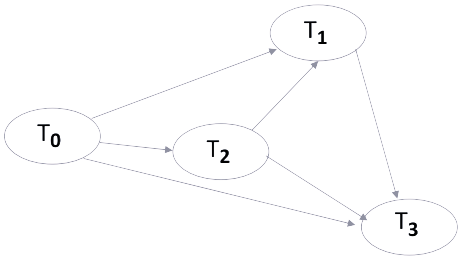
\includegraphics[width=0.5\linewidth]{images/conflict.png}
        \end{figure}
        There are no cycles in the graph, so this means that the schedule is CSR. 
    \end{example}
    \begin{proof}[CSR implies acyclicity of the conflict graph]
        Consider a schedule $S$ in $CSR$. As such, it is $\approx_C$ to a serial schedule. 
        Without loss of generality we can label the transactions of $S$ to say that their order in the serial schedule is: $T_1 T_2 \dots T_n$.
        Since the serial schedule has all conflicting pairs in the same order as schedule $S$, in the conflict graph there can only be arcs $(i,j)$, with $i<j$. 
        Then the graph is acyclic, as a cycle requires at least an arc $(i,j)$ with $i>j$.
    \end{proof}
    \begin{proof}[acyclicity of the conflict graph implies CSR]
        If $S$'s graph is acyclic then it induces a topological (partial) ordering on its nodes. The same partial order exists on the transactions of $S$. 
        Any serial schedule whose transactions are ordered according to the partial order is conflict-equivalent to $S$, because for all conflicting pairs $(i,j)$ it is always $i<j$. 
    \end{proof}
        
    \section{Concurrency control in practice}
    Conflict-serializability checking would be efficient if we knew the graph from the beginning, but usually we don't. Therefore, a scheduler must rather work online. 
    So, it is not feasible to maintain the conflict graph, update it, and check its acyclicity at each operation request. At the same time, the assumption that concurrency control 
    can work only with the commit-projection of the schedule is unrealistic because aborts do occur. We need some simple online decision criterion for the scheduler, which must 
    avoid as many anomalies as possible, and have negligible overhead. 
        
    When dealing with online concurrency control, it is important also to consider arrival sequences. The concurrency control system maps an arrival sequence into an effective a 
    posteriori schedule. To implement this online scheduling we use two main families of techniques:
    \begin{itemize}
        \item Pessimistic (locks): if a resource is taken, make the requester wait or pre-empt the holder.
        \item Optimistic (timestamps and versions): serve as many requests as possible, possibly using out-of-date versions of the data. 
    \end{itemize}
    Usually, commercial systems take the best of both worlds. 

    \section{Locking}
    The method called locking is the most used in commercial systems. A transaction is well-formed with respect to locking if: 
    \begin{itemize}
        \item Read operations are preceded by $r\_lock$ (shared) and followed by unlock. 
        \item Write operations are preceded by $w\_lock$ (exclusive) and followed by unlock. 
    \end{itemize}
    In both cases unlocking can be delayed with respect to the end of the operations. So, every object can be: free, r-locked or w-locked. 

    Transactions that first read and then write an object may acquire a $w\_lock$ already when reading or acquire a $r\_lock$ first and then upgrade it into a $w\_lock$ (escalation).

    The lock manager receives requests from the transactions and grants resources according to the conflict table: 

    \begin{table}[H]
        \centering
        \begin{tabular}{cccc}
        \textbf{}                              & \multicolumn{3}{c}{\textbf{Resource status}}                                                                                                                                                                                                   \\ \cline{2-4} 
        \multicolumn{1}{c|}{\textbf{Request}}  & \multicolumn{1}{c|}{\textit{FREE}}                                          & \multicolumn{1}{c|}{\textit{R\_LOCKED}}                                            & \multicolumn{1}{c|}{\textit{W\_LOCKED}}                                     \\ \hline
        \multicolumn{1}{|c|}{\textit{r\_lock}} & \multicolumn{1}{c|}{\begin{tabular}[c]{@{}c@{}}\checkmark\\ R\_LOCKED\end{tabular}} & \multicolumn{1}{c|}{\begin{tabular}[c]{@{}c@{}}\checkmark\\ R\_LOCKED($n++$)\end{tabular}} & \multicolumn{1}{c|}{\begin{tabular}[c]{@{}c@{}}\tikzxmark\\ W\_LOCKED\end{tabular}} \\ \hline
        \multicolumn{1}{|c|}{\textit{w\_lock}} & \multicolumn{1}{c|}{\begin{tabular}[c]{@{}c@{}}\checkmark\\ W\_LOCKED\end{tabular}} & \multicolumn{1}{c|}{\begin{tabular}[c]{@{}c@{}}\tikzxmark\\ R\_LOCKED\end{tabular}}        & \multicolumn{1}{c|}{\begin{tabular}[c]{@{}c@{}}\tikzxmark\\ W\_LOCKED\end{tabular}} \\ \hline
        \multicolumn{1}{|c|}{\textit{unlock}}  & \multicolumn{1}{c|}{ERROR}                                                  & \multicolumn{1}{c|}{\begin{tabular}[c]{@{}c@{}}\checkmark\\ $n--$\end{tabular}}            & \multicolumn{1}{c|}{\begin{tabular}[c]{@{}c@{}}\checkmark\\ FREE\end{tabular}}      \\ \hline
        \end{tabular}
    \end{table}

    \begin{example}
        Given a schedule with three transactions and the following operations: 
        \[r_1(x)w_1(x)r_2(x)r_3(y)w_1(y)\]
        We have the following locks: 
        \begin{itemize}
            \item $r_1(x)$: $r_1\_lock(x)$ request $\rightarrow$ Ok $\rightarrow$ $x$ is $r-locked$ with $n_x=1$. 
            \item $w_1(x)$: $w_1\_lock(x)$ request $\rightarrow$ Ok $\rightarrow$ $x$ is $w-locked$. 
            \item $r_2(x)$: $r_1\_lock(x)$ request $\rightarrow$ No, because $x$ is $w-locked$ $\rightarrow$ $T_2$ waits. 
            \item $r_3(y)$: $r_3\_lock(y)$ request $\rightarrow$ Ok $\rightarrow$ $y$ is $r-locked$ with $n_y=1$ and then $T_3$ unlocks $y$. 
            \item $w_1(y)$: $w_1\_lock(y)$ request $\rightarrow$ Ok $\rightarrow$ $y$ is $w-locked$ and then $x$ and $y$ are freed. 
        \end{itemize}
        So, the schedule a posteriori will become: 
        \[r_1(x)w_1(x)r_3(y)w_1(y)r_2(x)\]
        and we have that the transaction two is delayed. 
    \end{example}
    The locking system is implemented via lock tables, which are hash tables indexing the lockable items via hashing and where each locked item has a linked list associated with it. 
    Every node in the linked list represents the transaction which requested for lock, the lock mode and the current status. Every new lock request for the data item is appended to 
    the list.

    \section{Two-phase locking}
    With the locking showed before we do not eliminate the anomalies caused by non-repeatable reads. To avoid this problem we can use a two-phase rule which requires that a 
    transaction cannot acquire any other lock after releasing one. So, we have a phase where the transaction acquires all the locks, a phase where it executes all operations and 
    a final phase of unlocking. 
    \begin{definition}
        The class of \emph{two-phase locking} is the set of all schedules generated by a scheduler that: 
        \begin{itemize}
            \item Only processes well-formed transactions. 
            \item Grant locks according to the conflict table. 
            \item Checks that all transactions apply the two-phase rule.             
        \end{itemize}
    \end{definition}
    We have that $2PL$ is a strict subset of $CSR$ and also that $2PL$ implies $CSR$. 
    \begin{proof}[2PL implies CSR]
        We assume that a schedule $S$ is $2PL$. Consider, for each transaction, the moment in which it holds all locks and is going to release the first one. 
        We sort the transactions by this temporal value and consider the corresponding serial schedule $S^{'}$. We want to prove by contradiction that $S$ is conflict-equivalent to 
        $S^{'}$: 
        \[S^{'}\approx_CS,\dots\]
        Consider a generic conflict $o_i \rightarrow o_j$ in $S^{'}$ with $o_i \in T_i$, $0_j \in T_j$, and $i<j$. 
        By definition of conflict, $o_i$ and $o_j$ address the same resource $r$, and at least one of them is write. The two operations cannot occur in reverse order of $S$. 
        This proves that all $2PL$ schedules are view-serializable. 
    \end{proof}
    The anomalies that remain in this state are only the phantom inserts (needs predicate locks) and the dirty reads. 

    \section{Strict two-phase and predicate locking}
    \begin{definition}
        In \emph{strict two-phase locking} (or long duration locks) we also have that locks held by a transaction can be released only after commit or rollback.
    \end{definition}
    This version of locking is used in most commercial DBMS whenever a high level of isolation is required. 

    To prevent phantom inserts a lock should be placed also on future data using the predicate locks. If the predicate lock is on a resource, other transactions cannot insert, delete, 
    or update any tuple satisfying this predicate. 

    \section{Isolation levels in SQL '99}
    SQL defines transaction isolation levels which specify the anomalies that should be prevented by running at that level:

    \begin{table}[H]
        \centering
        \resizebox{\textwidth}{!}{%
        \begin{tabular}{c|ccc|}
        \cline{2-4}
                                                        & \textbf{Dirty read} & \textbf{Non-repeatable read} & \textbf{Phantoms}    \\ \hline
        \multicolumn{1}{|c|}{\textbf{Read uncommitted}} & $\checkmark$        & $\checkmark$                 & $\checkmark$         \\
        \multicolumn{1}{|c|}{\textbf{Read committed}}   & $\tikzxmark$        & $\checkmark$                 & $\checkmark$         \\
        \multicolumn{1}{|c|}{\textbf{Repeatable reads}}  & $\tikzxmark$        & $\tikzxmark$                 & $\checkmark$(insert) \\
        \multicolumn{1}{|c|}{\textbf{Serializable}}     & $\tikzxmark$        & $\tikzxmark$                 & $\tikzxmark$         \\ \hline
        \end{tabular}%
        }
    \end{table}
    The four levels are implemented respectively with: no read locks, normal read locks, strict read locks, and strict locks with predicate locks. Serializable is not the default 
    because its strictness can arise the following problems: 
    \begin{itemize}
        \item Deadlock: two or more transactions in endless mutual wait. 
        \item Starvation: a single transaction in endless wait. 
    \end{itemize}

    \section{Deadlocks}
    A deadlock occurs because concurrent transactions hold and in turn request resources held by other transactions. 
    \begin{definition}
        A \emph{lock graph} is a bipartite graph in which nodes are resources or transactions and arcs are lock requests or lock assignments. 

        A \emph{wait-for graph} is a graph in which nodes are transactions and arcs are waits for relationships. 
    \end{definition}
    A deadlock is represented by a cycle in the wait-for graph of transactions. 
    \begin{figure}[H]
        \centering
        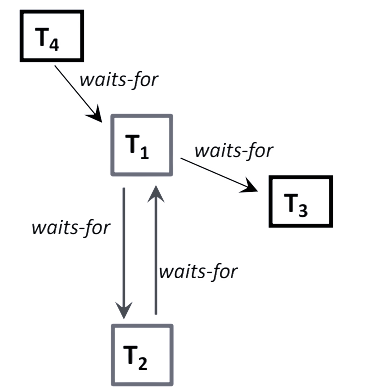
\includegraphics[width=0.35\linewidth]{images/waitgraph.png}
        \caption{An example of deadlock in the wait-for graph}
    \end{figure}
    It is possible to solve deadlocks in three different ways: 
    \begin{itemize}
        \item Timeout: a transaction is killed and restarted after a given amount of waiting, to be determined by the system manager. 
        \item Deadlock prevention: kills transactions that could cause cycles. It is implemented in two ways: 
            \begin{enumerate}
                \item Resource-based prevention puts restrictions on lock requests. The idea is that every transaction requests all resources at once, and only once. The main problem
                    is that it's not easy for transactions to anticipate all requests. 
                \item Transaction-based prevention puts restrictions on transactions' IDs. Assigning IDs to transactions incrementally allows to give an age to each one. It is 
                    possible to choose to kill the holding transaction (preemptive) or the requesting one (non-preemptive). The main problem is that the number of killings is too big. 
            \end{enumerate}
        \item Deadlock detection: it can be implemented with various algorithms and used for distributed resources. 
    \end{itemize}
    \begin{definition}
        The \emph{distributed dependency graph} is a wait-for graph where external call nodes represent a sub-transaction activating another sub-transaction at a different node. 
    \end{definition}
    The arrow shows a wait-for relation among local transactions. If one term is an external call, either the source is waited for by a remote transaction or waits for a remote 
    transaction. The Obermarck's algorithm needs the following assumptions: 
    \begin{itemize}
        \item Transactions execute on a single main node. 
        \item Transactions may be decomposed in sub-transactions running on other nodes. 
        \item When a transaction spawns a sub-transaction it suspends work until the latter completes. 
        \item Two wait-for relationships:
            \begin{itemize}
                \item $T_i$ waits for $T_j$ on the same node because $T_i$ needs a datum locked by $T_j$. 
                \item A sub-transaction of $T_i$ waits for another sub-transaction of $T_i$ running on a different node. 
            \end{itemize}
    \end{itemize}
    The goal of this algorithm is to detect a potential deadlock looking only at the local view of a node. Nodes exchange information and update their local graph based on the 
    received information. Node $A$ sends its local info to a node $B$ only if: it contains a transaction $T_i$ that is waited for from another remote transaction and waits for a 
    transaction $T_j$ active on $B$ and $i>j$.
    \begin{example}
        Given the following distributed dependency graph: 
        \begin{figure}[H]
            \centering
            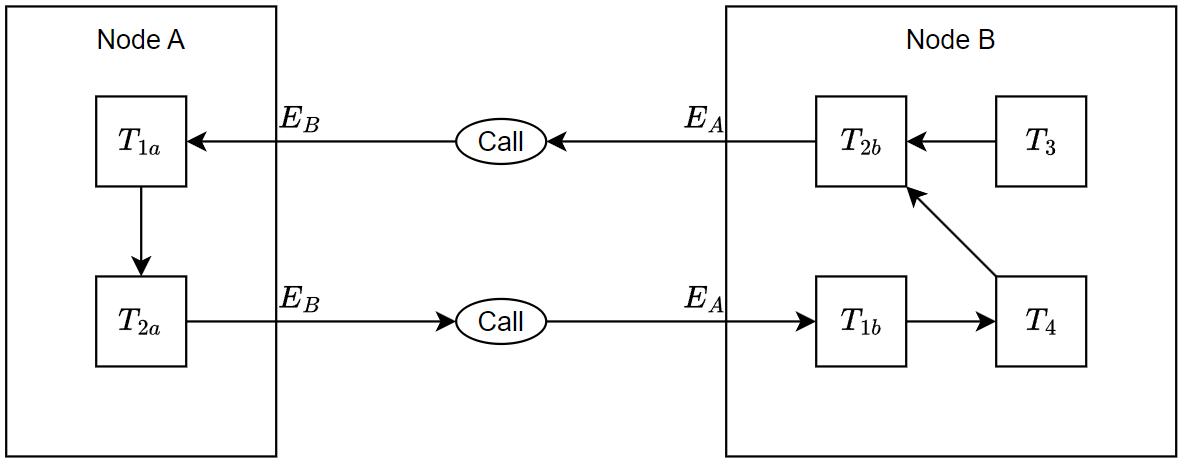
\includegraphics[width=0.5\linewidth]{images/distributedgraph.png}
        \end{figure}
        We can see that the potential deadlock is given by cycles. In this case, we have that $T_{2a}$ waits for $T_{1a}$ (data lock) that waits for $T_{1b}$ (call) that waits for 
        $T_{2b}$ (data locks) that waits for $T_{2a}$ (call). 
        
        In this case the node $A$ dispatches information to $B$, in fact we have $ E_b \rightarrow T_2 \rightarrow T_1 \rightarrow E_b$ and node $B$ cannot dispatch information to 
        $A$, because the forwarding rule is not respected: $E_a \rightarrow T_1 \rightarrow T_2 \rightarrow E_a$. 
    \end{example}
    The Obermarck's algorithm runs periodically at each node and consists in four steps: 
    \begin{enumerate}
        \item Get graph info from the previous nodes.
        \item Update the local graph by merging the received information. 
        \item Check the existence of cycles among transactions denoting potential deadlocks: if found, select one transaction in the cycle and kill it. 
        \item Send updated graph info to the next nodes. 
    \end{enumerate}
    \begin{example}
        Given the following distributed system:
        \begin{figure}[H]
            \centering
            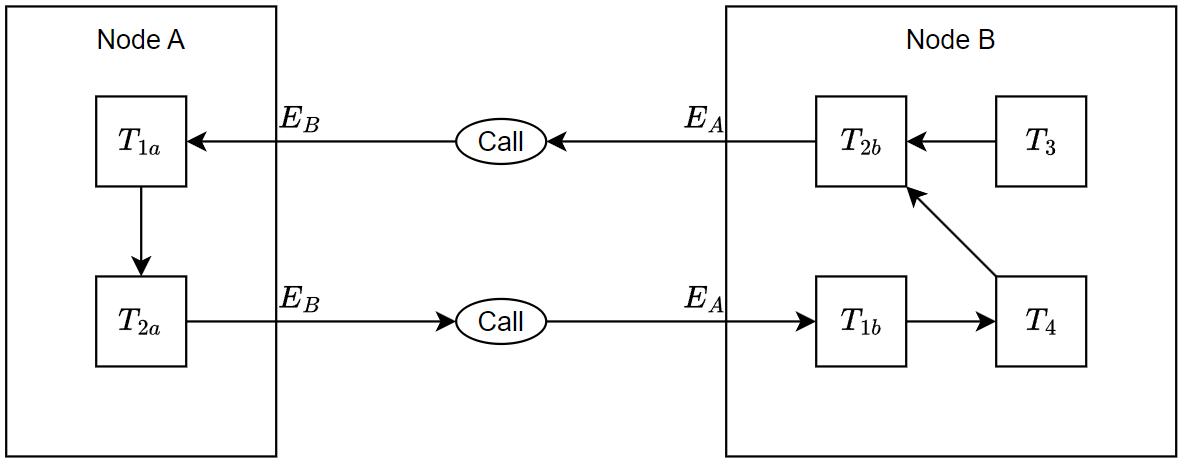
\includegraphics[width=0.5\linewidth]{images/distributedgraph.png}
        \end{figure}
        We want to apply the Obermarck's algorithm: 
        \begin{enumerate}
            \item Use the forwarding rule, in this case we have: 
                \begin{itemize}
                    \item At Node $A$: $E_b \rightarrow T_2 \rightarrow T_1 \rightarrow E_b$ info sent to Node $B$
                    \item At Node $B$: $E_a \rightarrow T_1 \rightarrow T_2 \rightarrow E_a$ info not sent $(i<j)$. 
                \end{itemize}
            \item At node $B$ there is the updated info $E_b \rightarrow T_2 \rightarrow T_1 \rightarrow E_b$ and it is added to the wait-for graph.
            \item At node $B$ a deadlock is detected (cycle between $T_1$ and $T_2$) and $T_1$, $T_2$ or $T_4$ are killed. 
            \item Updated information are sent to all nodes. 
        \end{enumerate}
    \end{example}
    There are four variants of this algorithm, based on various conventions.
    \begin{table}[H]
        \centering
        \begin{tabular}{c|cc|}
        \cline{2-3}
        \textbf{}               & \textbf{Message condition} & \textbf{Message receiver} \\ \hline
        \multicolumn{1}{|l|}{A} & $i>j$                      & Following node            \\
        \multicolumn{1}{|l|}{B} & $i>j$                      & Preceding node            \\
        \multicolumn{1}{|l|}{C} & $i<j$                      & Following node            \\
        \multicolumn{1}{|l|}{D} & $i<j$                      & Preceding node            \\ \hline
        \end{tabular}
    \end{table}
    In practice, the probability of deadlocks ($n^{-2}$) is much less than the conflict probability ($n^{-1}$). There are techniques to limit the frequency of deadlocks: 
    \begin{itemize}
        \item Update lock: the most frequent deadlock occurs when two concurrent transactions start by reading the same resources and then decide to write and try to upgrade their 
        lock to write on the resource. To avoid this situation, systems offer the update lock, that is used by transactions that will read and then write. The lock table become: 
        \begin{table}[H]
            \centering
            \begin{tabular}{ccccc}
            \textbf{}                                     & \multicolumn{4}{c}{\textbf{Resource status}}                                                                                                        \\ \cline{2-5} 
            \multicolumn{1}{c|}{\textbf{Request}}         & \textit{FREE}                     & \textit{SHARED}                   & \textit{UPDATE}                   & \multicolumn{1}{c|}{\textit{EXCLUSIVE}} \\ \hline
            \multicolumn{1}{|c|}{\textit{Shared lock}}    & \multicolumn{1}{c|}{$\checkmark$} & \multicolumn{1}{c|}{$\checkmark$} & \multicolumn{1}{c|}{$\checkmark$} & \multicolumn{1}{c|}{$\tikzxmark$}       \\ \hline
            \multicolumn{1}{|c|}{\textit{Update lock}}    & \multicolumn{1}{c|}{$\checkmark$} & \multicolumn{1}{c|}{$\checkmark$} & \multicolumn{1}{c|}{$\tikzxmark$} & \multicolumn{1}{c|}{$\tikzxmark$}       \\ \hline
            \multicolumn{1}{|c|}{\textit{Exclusive lock}} & \multicolumn{1}{c|}{$\checkmark$} & \multicolumn{1}{c|}{$\tikzxmark$} & \multicolumn{1}{c|}{$\tikzxmark$} & \multicolumn{1}{c|}{$\tikzxmark$}       \\ \hline
            \end{tabular}
        \end{table}
        \item Hierarchical lock: locks can be specified with different granularities. The objective of this is to lock the minimum amount of data and recognize conflicts as soon as
        possible. The method used to do so consists in asking locks on hierarchical resources by requesting resources top-down until the right level is obtained and releasing 
        locks bottom-up. This is done by using five locking modes: shared, exclusive, ISL (intention of locking a sub-element of the current element in shared mode), IXL (intention 
        of locking a sub-element of the current element in exclusive mode), and SIXL (lock of the element in shared mode with intention of locking a sub-element in exclusive mode). 
        The lock table become: 
        \begin{table}[H]
            \centering
            \begin{tabular}{ccccccc}
            \textbf{}                             & \multicolumn{6}{c}{\textbf{Resource status}}                                                                                                                                                                            \\ \cline{2-7} 
            \multicolumn{1}{c|}{\textbf{Request}} & \multicolumn{1}{c|}{\textit{FREE}} & \multicolumn{1}{c|}{\textit{ISL}} & \multicolumn{1}{c|}{\textit{IXL}} & \multicolumn{1}{c|}{\textit{SL}}  & \multicolumn{1}{c|}{\textit{SIXL}} & \multicolumn{1}{c|}{\textit{XL}}  \\ \hline
            \multicolumn{1}{|c|}{\textit{ISL}}    & \multicolumn{1}{c|}{$\checkmark$}  & \multicolumn{1}{c|}{$\checkmark$} & \multicolumn{1}{c|}{$\checkmark$} & \multicolumn{1}{c|}{$\checkmark$} & \multicolumn{1}{c|}{$\checkmark$}  & \multicolumn{1}{c|}{$\tikzxmark$} \\ \hline
            \multicolumn{1}{|c|}{\textit{IXL}}    & \multicolumn{1}{c|}{$\checkmark$}  & \multicolumn{1}{c|}{$\checkmark$} & \multicolumn{1}{c|}{$\checkmark$} & \multicolumn{1}{c|}{$\tikzxmark$} & \multicolumn{1}{c|}{$\tikzxmark$}  & \multicolumn{1}{c|}{$\tikzxmark$} \\ \hline
            \multicolumn{1}{|c|}{\textit{SL}}     & \multicolumn{1}{c|}{$\checkmark$}  & \multicolumn{1}{c|}{$\checkmark$} & \multicolumn{1}{c|}{$\tikzxmark$} & \multicolumn{1}{c|}{$\checkmark$} & \multicolumn{1}{c|}{$\tikzxmark$}  & \multicolumn{1}{c|}{$\tikzxmark$} \\ \hline
            \multicolumn{1}{|c|}{\textit{SIXL}}   & \multicolumn{1}{c|}{$\checkmark$}  & \multicolumn{1}{c|}{$\checkmark$} & \multicolumn{1}{c|}{$\tikzxmark$} & \multicolumn{1}{c|}{$\tikzxmark$} & \multicolumn{1}{c|}{$\tikzxmark$}  & \multicolumn{1}{c|}{$\tikzxmark$} \\ \hline
            \multicolumn{1}{|c|}{\textit{XL}}     & \multicolumn{1}{c|}{$\checkmark$}  & \multicolumn{1}{c|}{$\tikzxmark$} & \multicolumn{1}{c|}{$\tikzxmark$} & \multicolumn{1}{c|}{$\tikzxmark$} & \multicolumn{1}{c|}{$\tikzxmark$}  & \multicolumn{1}{c|}{$\tikzxmark$} \\ \hline
            \end{tabular}
        \end{table}
        \begin{example}
            Given a table $X$ with eight tuples divided in two pages: 
            \begin{table}[H]
                \centering
                \begin{tabular}{cc}
                \textbf{P1}                 & \textbf{P2}               \\ \hline
                \multicolumn{1}{|c|}{$t1$}  & \multicolumn{1}{c|}{$t5$} \\ \hline
                \multicolumn{1}{|c|}{$t2$}  & \multicolumn{1}{c|}{$t6$} \\ \hline
                \multicolumn{1}{|c|}{$t3$}  & \multicolumn{1}{c|}{$t7$} \\ \hline
                \multicolumn{1}{|c|}{$t4$}  & \multicolumn{1}{c|}{$t8$} \\ \hline
                \end{tabular}
            \end{table}
            And two transactions with the following schedules: 
            \[T_1=r(P1)\:w(t3)\:r(t8)\]
            \[T_2=r(t2)\:r(t4)\:w(t5)\:w(t6)\]
            We can see that they are not in a read-write conflict (because they are independent of the order). Without hierarchical locking both transactions needs to operate on the 
            same table, so the concurrency will be almost useless in this case. But with this technique, calling $X$ the table, we have that the transaction acquires the following
            locks: 
            \[T_1:\:IXL(root)\:SIXL(P1)\:XL(t3)\:ISL(P2)\:SL(t8)\]
            \[T_2:\:IXL(root)\:ISL(P1)\:SL(t2)\:SL(t4)\:IXL(P2)\:XL(t5)\:XL(t6)\]
        \end{example}
    \end{itemize}

    \section{Timestamps}
    Locking is also named pessimistic concurrency control because it assumes that collisions will arise but in reality collisions are rare. 
    
    So, it is possible to use optimistic concurrency control methods like timestamps, which are identifier that defines a total ordering of the events of a system. Each transaction has a timestamp representing the time 
    at which the transaction begins so that transactions can be ordered: the smaller is the index the older is the transaction. A schedule is accepted only if it reflects the serial 
    ordering of the transactions induced by their timestamps. The timestamps are given by a system's function on request. The syntax of a timestamp is the following: 
    \[\textnormal{event-id}.\textnormal{node-id}\]
    The algorithm's synchronization is based on send-receive of messages, and it is called Lamport method: it is not possible to receive a message 
    from the future, if this happens the bumping rule is used to bump the timestamp of the receive event beyond the timestamp of the send event.     
    \begin{example}
        An example of timestamps assignation at two different nodes can be the following. 
        \begin{figure}[H]
            \centering
            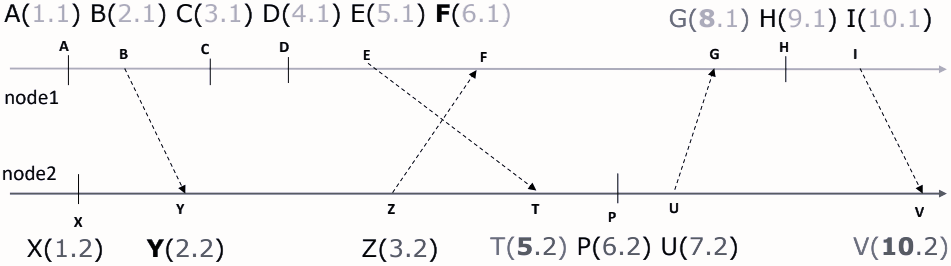
\includegraphics[width=0.75\linewidth]{images/timestamps.png}
        \end{figure}
    \end{example}
    The scheduler uses two counters: one for writes WTM($x$) and another for reads RTM($x$). The scheduler receives read/write requests tagged with the timestamp of the 
    requesting transaction. In case of a read operation we can have: 
    \begin{itemize}
        \item If $ts<\textnormal{WTM}(x)$ the request is rejected and the transaction is killed. 
        \item Else, access is granted, and we set $\textnormal{RTM}(x)=\max(\textnormal{RTM}(x),ts)$. 
    \end{itemize}
    In case of a write operation we can have: 
    \begin{itemize}
        \item If $ts<\textnormal{RTM}(x)$ or $ts<\textnormal{WTM}(x)$ the request is rejected, and the  transaction is killed. 
        \item Else, access is granted, and we set $\textnormal{WTM}(x)=ts$. 
    \end{itemize}
    The previous rules cause too many transaction killings. 
    \begin{example}
        Let us assume $\textnormal{RTM}(x)=7$ and $\textnormal{WTM}(x)=4$ and the following schedule: 
        \[S=r_6(x) r_8(x) r_9(x) w_8(x) w_{11}(x) r_{10}(x)\]
        Using the timestamps we obtain: 
        \begin{table}[H]
            \centering
            \begin{tabular}{ccc}
            \textbf{Request} & \textbf{Response} & \textbf{New value} \\ \hline
            $r_6(x)$         & $\checkmark$      & -                  \\
            $r_8(x)$         & $\checkmark$      & $\textnormal{RTM}(x)=8$         \\
            $r_9(x)$         & $\checkmark$      & $\textnormal{RTM}(x)=9$         \\
            $w_8(x)$         & $\tikzxmark$      & $T_8$ killed       \\
            $w_{11}(x)$      & $\checkmark$      & $\textnormal{WTM}(x)=11$        \\
            $r_{10}(x)$      & $\tikzxmark$      & $T_{10}$ killed   
            \end{tabular}
        \end{table}
    \end{example}
    It is not possible to compare 2PL to TS (this means that there is no subset between the categories). We have only that TS implies CSR. 
    \begin{proof}[TS implies CSR]
        Let $S$ be a TS schedule of $T_1$ and $T_2$. Suppose $S$ is not CSR, which implies that it contains a cycle between $T_1$ and $T_2$. $S$ contains $op_1(x)$, $op_2(x)$ where at 
        least one is a write. $S$ contains also $op_2(y)$, $op_1(y)$ where at least one is a write. 
        When $op_1(y)$ arrives:
        \begin{itemize}
            \item If $op_1(y)$ is a read, $T_1$ is killed by TS because it tries to read a value written by a younger transaction, so it is a contradiction. 
            \item If $op_1(y)$ is a write, $T_1$ is killed no matter what $op_2(y)$ is, because it tries to write a value already read or written by a younger transaction, so it is a 
                contradiction. 
        \end{itemize}
    \end{proof}
    Basic TS-based control considers only committed transactions in the schedule, aborted transactions are not considered. If aborts occur, dirty reads may happen. To cope with dirty 
    reads, a variant of basic TS must be used: a transaction $T_i$ that issues $r_{ts}(x)$ or $w_{ts}(x)$ such that $ts>\textnormal{WTM}(x)$ has its read or write operation delayed until the
    transaction $T^{'}$ that wrote the value of $x$ has committed or aborted. This is similar to long duration write locks. 
    \begin{table}[H]
        \centering
        \begin{tabular}{c|cc}
        \textbf{Action} & \textbf{2PL}          & \textbf{TS}          \\ \hline
        Transaction     & Wait                  & Killed and restarted \\
        Serialization   & Imposed by conflicts  & Imposed by timestamp \\
        Delay           & Long (strict version) & Long                 \\
        Deadlocks       & Possible              & Prevented           
        \end{tabular}
    \end{table}
    Since that restarting a transaction is costlier than waiting, 2PL is better if used alone. Commercial system mediates between those techniques to get the better feature from both. 
    To reduce the number of killings it is possible to use the Thomas rule, that changes the rule for the write operations: 
    \begin{itemize}
        \item If $ts<\textnormal{RTM}(x)$ the request is rejected and the transaction is killed. 
        \item If $ts<\textnormal{WTM}(x)$ then our write is obsolete: it can be skipped. 
        \item Else, access is granted, and we set $\textnormal{WTM}(x)=ts$. 
    \end{itemize}

    \section{Multi-version timestamps}
    The idea of multi-version is that writes generate new versions, and that reads access the right version. Writes generate new copies, each one with a new WTM, so each object $x$ 
    always has $N \geq 1$ active versions. There is a unique global RTM($x$). Old versions are discarded when there are no transactions that need their values. 
    In theory, it is possible to use the following rule: 
    \begin{itemize}
        \item $r_{ts}(x)$ is always accepted. A copy $x_k$ is selected for reading such that:
            \begin{itemize}
                \item If $ts \geq \textnormal{WTM}_N(x)$, then $k=N$.
                \item Else take $k$ such that $\textnormal{WTM}_k(x) \leq ts < \textnormal{WTM}_{k+1}(x)$. 
            \end{itemize}
        \item $w_{ts}(x)$: 
            \begin{itemize}
                \item If $ts < \textnormal{RTM}(x)$ the request is rejected. 
                \item Else a new version is created for timestamp $ts$ ($N$ is incremented). 
            \end{itemize}
    \end{itemize}
    \begin{example}
        Let us assume $\textnormal{RTM}(x)=7$, $N=1$ and $\textnormal{WTM}_1(x)=4$ and the following schedule: 
        \[S=r_6(x) r_8(x) r_9(x) w_8(x) w_{11}(x) r_{10}(x) r_{12}(x) w_{14}(x) w_{13}(x)\]
        Using the multi-version we obtain: 
        \begin{table}[H]
            \centering
            \begin{tabular}{ccc}
            \textbf{Request} & \textbf{Response}         & \textbf{New value}  \\ \hline
            $r_6(x)$         & $\checkmark$              & -                   \\
            $r_8(x)$         & $\checkmark$              & $\textnormal{RTM}(x)=8$          \\
            $r_9(x)$         & $\checkmark$              & $\textnormal{RTM}(x)=9$          \\
            $w_8(x)$         & $\tikzxmark$              & $T_8$ killed        \\
            $w_{11}(x)$      & $\checkmark$              & $\textnormal{WTM}_2(x)=11,\:N=2$ \\
            $r_{10}(x)$      & $\checkmark$ on $x_{(1)}$ & $\textnormal{RTM}(x)=10$         \\
            $r_{12}(x)$      & $\checkmark$ on $x_{(2)}$ & $\textnormal{RTM}(x)=12$         \\
            $w_{14}(x)$      & $\checkmark$              & $\textnormal{WTM}_3(x)=14,\:N=3$ \\
            $w_{13}(x)$      & $\checkmark$              & $\textnormal{WTM}_4(x)=14,\:N=4$
            \end{tabular}
        \end{table}
    \end{example}

    In practice, it is possible to use the following rule: 
    \begin{itemize}
        \item $r_{ts}(x)$ is always accepted. A copy $x_k$ is selected for reading such that:
            \begin{itemize}
                \item If $ts \geq \textnormal{WTM}_N(x)$, then $k=N$. 
                \item Else take $k$ such that $\textnormal{WTM}_k(x) \leq ts < \textnormal{WTM}_{k+1}(x)$. 
            \end{itemize}
        \item $w_{ts}(x)$:
            \begin{itemize}
                \item If $ts < \textnormal{RTM}(x)$ or $ts < \textnormal{WTM}_N(x)$ the request is rejected. 
                \item Else a new version is created for timestamp $ts$ ($N$ is incremented)
            \end{itemize}
    \end{itemize}
    \begin{example}
        Let us assume $\textnormal{RTM}(x)=7$, $N=1$ and $\textnormal{WTM}_1(x)=4$ and the following schedule: 
        \[S=r_6(x) r_8(x) r_9(x) w_8(x) w_{11}(x) r_{10}(x) r_{12}(x) w_{14}(x) w_{13}(x)\]
        Using the multi-version we obtain: 
        \begin{table}[H]
            \centering
            \begin{tabular}{ccc}
            \textbf{Request} & \textbf{Response}         & \textbf{New value}  \\ \hline
            $r_6(x)$         & $\checkmark$              & -                   \\
            $r_8(x)$         & $\checkmark$              & $\textnormal{RTM}(x)=8$          \\
            $r_9(x)$         & $\checkmark$              & $\textnormal{RTM}(x)=9$          \\
            $w_8(x)$         & $\tikzxmark$              & $T_8$ killed        \\
            $w_{11}(x)$      & $\checkmark$              & $\textnormal{WTM}_2(x)=11,\:N=2$ \\
            $r_{10}(x)$      & $\checkmark$ on $x_{(1)}$ & $\textnormal{RTM}(x)=10$         \\
            $r_{12}(x)$      & $\checkmark$ on $x_{(2)}$ & $\textnormal{RTM}(x)=12$         \\
            $w_{14}(x)$      & $\checkmark$              & $\textnormal{WTM}_3(x)=14,\:N=3$ \\
            $w_{13}(x)$      & $\tikzxmark$              & $T_{13}$ killed
            \end{tabular}
        \end{table}
    \end{example}
    \subsection{Isolation level introduced with TS-multi}
    The realization of TS-multi gives the opportunity to introduce into the DBMS another isolation level called snapshot isolation. In this level only WTM($x$) is used. The rule 
    used in this level states that every transaction reads the version consistent with its timestamp, and defers writes to the end. If the scheduler detects that the writes of a
    transaction conflict with writes of other concurrent transactions after the snapshot timestamp, it aborts. Snapshot isolation does not guarantee serializability: it is possible 
    to have a new anomaly called write skew (non-determinism). 
    
    \section{Concurrency classes sets}
    The final structure for the sets is the following. 
    \begin{figure}[H]
        \centering
        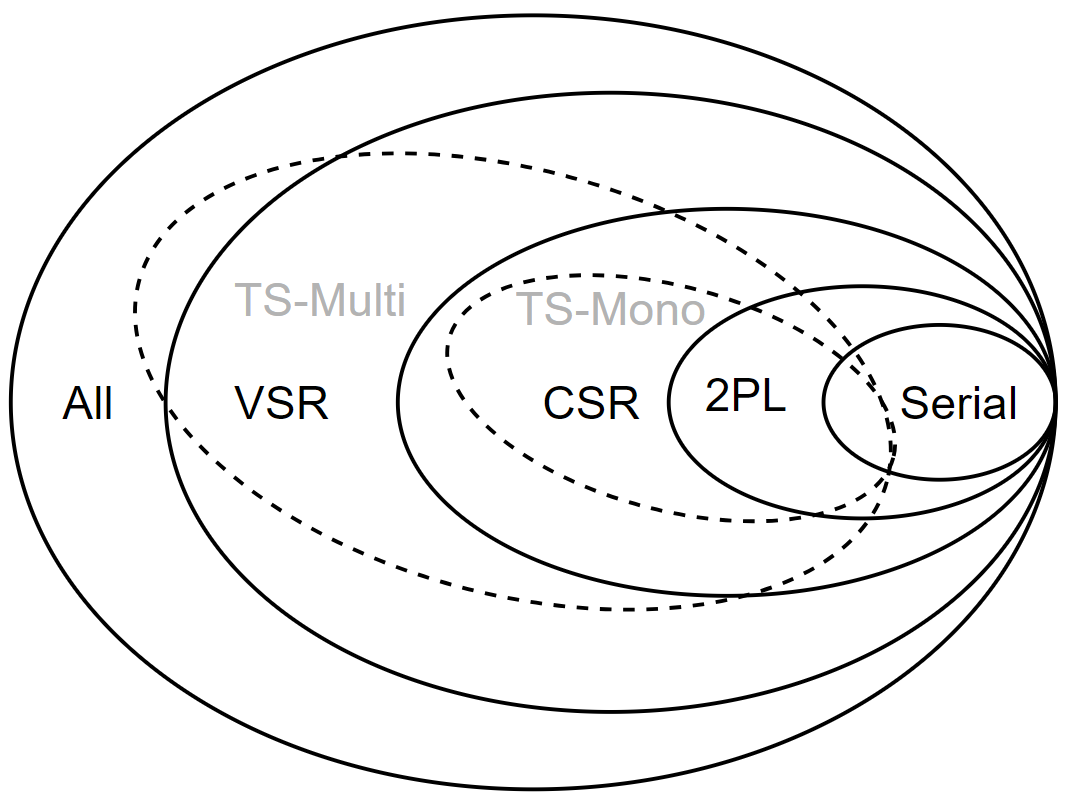
\includegraphics[width=1\linewidth]{images/set.png}
    \end{figure}
    
\newpage 

\chapter{Ranking}
    \section{Introduction}
    It is possible to create ranking to get the best result out of the data using the multi-objective optimization (simultaneous optimization of different criteria). 
    
    A general multi-objective problem can be formulated as follows: given $N$ objects described by $d$ attributes, we need to find the best $k$ objects. 
    
    The main approaches to solve the multi-objective optimization are: 
    \begin{itemize}
        \item Ranking queries: selects the top $k$ objects according to a given scoring function.
        \item Skyline queries: selects the set of non-dominated objects. 
    \end{itemize}

    \section{History}
    In the $13^{\textnormal{th}}$ century this problem was introduced with the elections polls. Borda proposed to give a number of penalty points equivalent to the position 
    of the electors in a voter's ranking, so the winner will be the candidate with the lowest overall penalty. Condorcet, instead, proposed to consider as winner the candidate who 
    defeats every other candidate in pairwise majority rule election.
    \begin{example}
        Given ten voters and three candidates with the following votes: 
        \begin{table}[H]
            \centering
            \begin{tabular}{|c|c|c|c|c|c|c|c|c|c|}
            \hline
            1 & 2 & 3 & 4 & 5 & 6 & 7 & 8 & 9 & 10 \\ \hline
            A & A & A & A & A & A & C & C & C & C  \\ 
            C & C & C & C & C & C & B & B & B & B  \\ 
            B & B & B & B & B & B & A & A & A & A  \\ \hline
            \end{tabular}
        \end{table}
        For Borda we have: 
        \begin{itemize}
            \item $A: 1 \cdot 6+3 \cdot 4 = 18$
            \item $B: 3 \cdot 6+2 \cdot 4 = 26$
            \item $C: 2 \cdot 6+1 \cdot 4 = 16$ (winner)
        \end{itemize}
        While for Condorcet we have that $A$ wins in pairwise majority. So, the winner depends on the method used. 
    \end{example}

    In 1950 Arrow proposed the axiomatic approach. He defined the aggregation as axioms and understood that a small set of natural requirements cannot be simultaneously achieved by 
    any nontrivial aggregation function. So, he stated the Arrow's paradox: no rank-order electoral system can be designed that always satisfies these fairness criteria:
    \begin{itemize}
        \item No dictatorship (nobody determines, alone, the group's preference). 
        \item If all prefer $X$ to $Y$, then the group prefers $X$ to $Y$. 
        \item If, for all voters, the preference between $X$ and $Y$ is unchanged, then the group preference between $X$ and $Y$ is unchanged. 
    \end{itemize}

    To solve this paradox, in the later years researchers tried to measure the values of all analyzed objects and created the metric approach. This consist in finding a new ranking 
    $R$ whose total distance to the initial rankings $R_1,\dots,R_n$ is minimized. The distance between rankings can be found in several ways: 
    \begin{itemize}
        \item Kendall tau distance $K(R_1, R_2)$, defined as the number of exchanges in a bubble sort to convert $R_1$ to $R_2$. 
        \item Spearman's foot-rule distance $F(R_1, R_2)$, which adds up the distance between the ranks of the same item in the two rankings. 
    \end{itemize}
    Finding an exact solution is computationally hard for Kendall tau (NP-complete), but tractable for Spearman's foot-rule (P time). These distances are related:
    \[K(R_1, R_2) \leq F(R_1, R_2) \leq 2K(R_1, R_2)\]
    And it is possible to find efficient approximation for $F(R_1, R_2)$. 

    \section{Opaque rankings}
    The opaque rankings consider only the position and no other associated score. The algorithm called MedRank is based on the notion of 
    median and provides an approximation of the foot-rule optimal aggregation. The inputs of this algorithm are: an integer $k$, and a ranked list 
    $R_1,\dots,R_m$ of $N$ elements. The output is the top $k$ elements according to median ranking. The idea of the algorithm is the following: 
    \begin{enumerate}
        \item Use sorted accesses in each list, one element at a time, until there are $k$ elements that occur in more than $m/2$ lists.
        \item These are the top $k$ elements. 
    \end{enumerate}
    \begin{definition}
        The maximum number of sorted accesses made on each list is also called the \emph{depth reached} by the algorithm. 
    \end{definition}
    \begin{example}
        Suppose we have to sort the hotels based on three rankings criteria: price, rating, and distance. Using the MedRank algorithm we can make one sorted access at a time in 
        each ranking and then look for hotels that appear in at least two rankings. We assume that price, rating and distance are opaque. The 
        ranks of hotels are the following:
        \begin{table}[H]
            \centering
            \begin{tabular}{c|c|c}
            \textbf{Price} & \textbf{Rating} & \textbf{Distance} \\ \hline
            Ibis           & Crillon         & Le Roch           \\
            Etap           & Novotel         & Lodge In          \\
            Novotel        & Sheraton        & Ritz              \\
            Mercure        & Hilton          & Lutetia           \\
            Hilton         & Ibis            & Novotel           \\
            Sheraton       & Ritz            & Sheraton          \\
            Crillon        & Lutetia         & Mercure           \\
            $\dots$        & $\dots$         & $\dots$          
            \end{tabular}
        \end{table}
        If we use MedRank with $k=3$, we will obtain the following rank: 
        \begin{table}[H]
            \centering
            \begin{tabular}{cc}
            \hline
            \textbf{Top k hotels}       & \textbf{Median rank}          \\ \hline
            Novotel                     & median$\{2,3,5\}=3$           \\ 
            Hilton                      & median$\{4,5,?\}=5$           \\ 
            Ibis                        & median$\{1,5,?\}=5$           \\ \hline
            \end{tabular}
        \end{table}
        The depth in this case is equal to five. 
    \end{example}
    \begin{definition}
        An algorithm is \emph{optimal} if its execution cost is never worse than any other algorithm on any input.
    \end{definition}
    MedRank is not optimal, but it is instance optimal. This means that among the algorithms that access the lists in sorted order, this is the best possible algorithm on every 
    input instance. 
    \begin{definition}
        Let $\boldsymbol{A}$ be a family of algorithms, $\boldsymbol{I}$ a set of problem instances. Let cost be a cost metric applied to an algorithm-instance pair. Algorithm 
        $A^{*}$ is instance-optimal with respect to $\boldsymbol{A}$ and $\boldsymbol{I}$ for the cost metric cost if there exist constants $k_1$ and $k_2$ such that, for all 
        $A \in \boldsymbol{A}$ and $I \in \boldsymbol{I}$: 
        \[\textnormal{cost}(A^{*}, I) \leq k_1 \textnormal{cost}(A, I) + k_2\]
    \end{definition}
    If $A^{*}$ is instance-optimal, then any algorithm can improve with respect to $A^{*}$ by only a constant factor $r$, which is therefore called the optimality ratio of $A^{*}$. 
    Instance optimality is a much stronger notion than optimality in the average or worst case. 

    \section{Ranking queries}
    Ranking queries, also called top-$k$ queries, aim to retrieve only the $k$ best ansoftwareers from a potentially very large result set. Ranking is based on ordering objects based on their relevance.

    Assume a scoring function $S$ that assigns to each tuple $t$ a numerical score for ranking tuples. The algorithm needs these inputs: cardinality $k$, dataset $R$, and a scoring function $S$. The output is 
    the $k$ highest-scored tuples with respect to $S$. The idea is the following: 
    \begin{enumerate}
        \item For all tuples $t$ in $R$ compute $S(t)$. 
        \item Sort tuples based on their scores.
        \item Return the first $k$ highest-scored tuples. 
    \end{enumerate}
    This naïve approach is expensive for large dataset because it requires to sort a large amount of data. It is even worse if more than one relation is involved because it needs to join all tuples. So, 
    we now know that two abilities are required: 
    \begin{itemize}
        \item Ordering the tuples according to their scores. This is taken care of by 
            \begin{lstlisting}[style=SQL]
ORDER BY
            \end{lstlisting}
        \item Limiting the output cardinality to $k$ tuples. This is taken care of by 
            \begin{lstlisting}[style=SQL]
FETCH FIRST k ROWS ONLY
            \end{lstlisting}
    \end{itemize} 
    \begin{example}
        Consider the following queries: 
        \begin{lstlisting}[style=SQL]
a)  SELECT *
    FROM UsedCarsTable
    WHERE Vehicle = 'Audi/A4'
    AND Price <= 21000
    ORDER BY 0.8*Price+0.2*Miles
b)  SELECT *
    FROM UsedCarsTable
    WHERE Vehicle = 'Audi/A4'
    ORDER BY 0.8*Price+0.2*Miles
        \end{lstlisting}
        The values 0.8 and 0.2, also called weights, are a way to normalize our preferences on price and mileage.
        The first query will likely miss some relevant ansoftwareers (near-miss). The second query will return all Audi/A4 in the dataset (information overload).
    \end{example}
    Only the first $k$ tuples become part of the result. If more than one set of $k$ tuples satisfies the ordering directive, any of such sets is a valid ansoftwareer 
    (non-deterministic semantics). 

    To evaluate a top-$k$ query it is possible to consider two basic aspects: 
    \begin{itemize}
        \item Query type: one relation, many relations, and aggregate results. 
        \item Access paths: no index, indexes on all/some ranking attributes. 
    \end{itemize}
    In the simplest case, that is a top-$k$ selection query with only one relation, if the input is sorted according to $S$ it is possible to read only the first $k$ tuples; 
    If the tuples are not sorted we need to perform an in-memory sort (through the heap), that has a complexity of $O(N\log{k})$. 
    \begin{example}
        Consider the two-dimensional attribute space (Price, Mileage) of the previous example: 
        \begin{figure}[H]
            \centering
            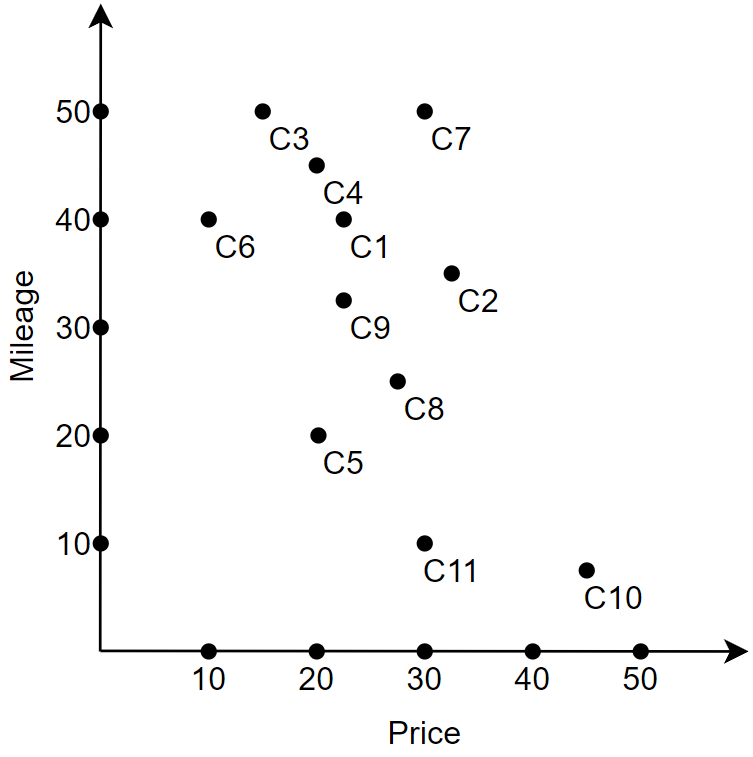
\includegraphics[width=0.25\linewidth]{images/ex1.png}
        \end{figure}
        In the image each tuple is represented by a two-dimensional point $(p, m)$, where $p$ is the Price and $m$ is the Mileage. Intuitively, minimizing
        $0.8\cdot Price + 0.2\cdot Mileage$ is equivalent to looking for points close to $(0,0)$. Our preferences are essential to determine the result. Consider the line of equation: 
        \[0.8\cdot Price + 0.2\cdot Mileage = v\]
        where $v$ is a constant. This can also be written as:
        \[Mileage = -4\cdot Price + 5\cdot v\]
        from which we see that all the lines have a slope $-4$. By definition, all the points of the same line are equally good. If we change the weights, it is possible 
        that the best choice also varies. 
        The target of a query is not necessarily $(0,0)$, rather it can be any point $q=(q_1,q_2)$. 
    \end{example}
    In general, in order to determine the goodness of a tuple $t$, we compute its distance from the target point $q$: the lower the distance from $q$, the better. 
    If we consider the distances the model become: 
    \begin{itemize}
        \item An $m$-dimensional $(m \geq 1)$ space $A = (A_1,A_2,\dots,A_m)$ of ranking attributes. 
        \item A relation $R(A_1,A_2,\dots,A_m,B_1,B_2,\dots)$, where $B_1,B_2,\dots$ are other attributes.
        \item A target point $q = (q_1,q_2,\dots,q_m)$, $q \in A$. 
        \item A function $d: A \times A \rightarrow \mathbb{R}^{+}$, measuring the distance between points in $A$. 
    \end{itemize}
    \begin{definition}
        The top-$k$ query is called $k$-\emph{nearest neighbors} if given a point $q$, a relation $R$, an integer $k \geq 1$, and a distance function $d$ it determines the $k$ tuples 
        in $R$ that are closest to $q$ according to $d$. 

        The distance function called $L_p$-\emph{norms} is defined as:
        \[L_p(t,q)=\left(\sum_{i=1}^{m}{\left\lvert t_i-q_i \right\rvert^{p}}\right)^{\frac{1}{p}}\]
    \end{definition}
    Relevant cases of the $L_p$-norm are: 
    \begin{itemize}
        \item Euclidean distance (ellipsoids): $L_2(t,q)=\sqrt{\sum_{i=1}^{m}{\left\lvert t_i-q_i \right\rvert^{2}}}$
        \item Manhattan distance (rhomboids): $L_1(t,q)=\sum_{i=1}^{m}{\left\lvert t_i-q_i \right\rvert}$
        \item Čebyšëv distance (rectangles): $L_{\infty}(t,q)=\max_{i}\{\left\lvert t_i-q_i\right\rvert\}$
    \end{itemize}
    The shape of the attribute space depends on the distance function and the weight associated to each coordinate: 
    \begin{itemize}
        \item Euclidean distance (hyper-ellipsoids):
            \[L_2(t,q;W)=\sqrt{\sum_{i=1}^{m}{w_i\left\lvert t_i-q_i \right\rvert^{2}}}\]
        \item Manhattan distance (hyper-rhomboids): 
            \[L_1(t,q;W)=\sum_{i=1}^{m}{w_i\left\lvert t_i-q_i \right\rvert}\]
        \item Čebyšëv distance (hyper-rectangles): 
            \[L_{\infty}(t,q;W)=\max_{i}\{w_i \left\lvert t_i-q_i\right\rvert\}\]
    \end{itemize}
    \begin{definition}
        In a \emph{top-$k$ join query} we have $n > 1$ input relations and a scoring function $S$ defined on the result of the join. The general formula is: 
        \begin{lstlisting}[style=SQL]
SELECT <attributes>
FROM R1,R2,...,Rn
WHERE <conditions>
ORDER BY S(p1,p2,...,pm) [DESC]
FETCH FIRST k ROWS ONLY             
        \end{lstlisting}
        where $p_1,p_2,\dots,p_m$ are the scoring criteria. 
    \end{definition}

    In the top-$k$ $1-1$ join queries all the joins are on a common key attribute. It is possible to have two main scenarios: 
    \begin{itemize}
        \item There is an index for retrieving tuples according to each preference. 
        \item The relation is spread over several sites, each providing information only on part of the objects.
    \end{itemize}
    We make the following assumptions: 
    \begin{itemize}
        \item Each input list supports sorted access: this means that each access returns the identifier of the next best object, its partial score $p_j$. 
        \item Each input list supports random access: this means that each access returns the partial score of an object, given its identifier. 
        \item The identifier of an object is the same across all inputs. 
        \item Each input consists of the same set of objects. 
    \end{itemize}
    \begin{example}
        Given the following reviews on two different sites: 
        \begin{table}[H]
            \centering
            \begin{tabular}{ccccc}
            \multicolumn{1}{l}{\textbf{EatWell}}     &                                     & $\:\:\:\:\:\:$                 & \multicolumn{1}{l}{\textbf{BreadAndWine}} &                                  \\ \cline{1-2} \cline{4-5} 
            \multicolumn{1}{|l}{\textbf{Name}}       & \multicolumn{1}{c|}{\textbf{Score}} & \multicolumn{1}{c|}{\textbf{}} & \multicolumn{1}{l}{\textbf{Name}}        & \multicolumn{1}{c|}{\textbf{Score}} \\ \cline{1-2} \cline{4-5} 
            \multicolumn{1}{|l}{The old mill}        & \multicolumn{1}{c|}{9.2}            & \multicolumn{1}{c|}{}          & \multicolumn{1}{l}{Da Gino}              & \multicolumn{1}{c|}{9.0}            \\
            \multicolumn{1}{|l}{The canteen}         & \multicolumn{1}{c|}{9.0}            & \multicolumn{1}{c|}{}          & \multicolumn{1}{l}{Cheers!}              & \multicolumn{1}{c|}{8.5}            \\  
            \multicolumn{1}{|l}{Cheers!}             & \multicolumn{1}{c|}{8.3}            & \multicolumn{1}{c|}{}          & \multicolumn{1}{l}{The old mill}         & \multicolumn{1}{c|}{7.5}            \\ 
            \multicolumn{1}{|l}{Da Gino}             & \multicolumn{1}{c|}{7.5}            & \multicolumn{1}{c|}{}          & \multicolumn{1}{l}{Chez Paul}            & \multicolumn{1}{c|}{7.5}            \\ 
            \multicolumn{1}{|l}{Let's eat!}          & \multicolumn{1}{c|}{6.4}            & \multicolumn{1}{c|}{}          & \multicolumn{1}{l}{The canteen}          & \multicolumn{1}{c|}{7.0}            \\ 
            \multicolumn{1}{|l}{Chez Paul}           & \multicolumn{1}{c|}{5.5}            & \multicolumn{1}{c|}{}          & \multicolumn{1}{l}{Los pollos hermanos}  & \multicolumn{1}{c|}{6.5}            \\ 
            \multicolumn{1}{|l}{Los pollos hermanos} & \multicolumn{1}{c|}{5.0}            & \multicolumn{1}{c|}{}          & \multicolumn{1}{l}{Let's eat!}           & \multicolumn{1}{c|}{6.0}            \\ \cline{1-2} \cline{4-5} 
            \end{tabular}
        \end{table}
        If we aggregate the two tables with the following query: 
        \begin{lstlisting}[style=SQL]
SELECT *
FROM EatWell EW, BreadAndWine BW
WHERE EW.Name = BW.Name
ORDER BY EW.Score + BW.Score DESC
FETCH FIRST 1 ROW ONLY 
        \end{lstlisting}
        We will obtain the following result: 
        \begin{table}[H]
            \centering
            \begin{tabular}{|lc|}
            \hline
            \textbf{Name}       & \textbf{Global score} \\ \hline
            Cheers!             & 16.8                  \\ \hline
            The old mill        & 16.7                  \\ \hline
            Da Gino             & 16.5                  \\ \hline
            The canteen         & 16.0                  \\ \hline
            Chez Paul           & 13.0                  \\ \hline
            Let's eat!          & 12.4                  \\ \hline
            Los pollos hermanos & 11.5                  \\ \hline
            \end{tabular}
        \end{table}
        Note that the winner is not the best locally. 
    \end{example}
    Each object o returned by the input $L_j$ has an associated local/partial score $p_j(o) \in [0,1]$. For convenience, scores are normalized. The hypercube $[0,1]^m$ 
    is called the score space. The point $p(o) = (p_1(o),p_2(o),\dots,p_m(o)) \in [0,1]^m$ is the map of $o$ into the score space. The global score $S(o)$ of $o$ is 
    computed by means of a scoring function $S$ that combines in some way the local scores of $o$:
    \[S(o) \equiv  S(p(o)) = S(p_1(o),p_2(o),\dots,p_m(o))\]
    with $S:[0,1]^m \rightarrow \mathbb{R}^{+}$. 
    \begin{example}
        Consider the attribute space $A = (Price,Mileage)$
        \begin{figure}[H]
            \centering
            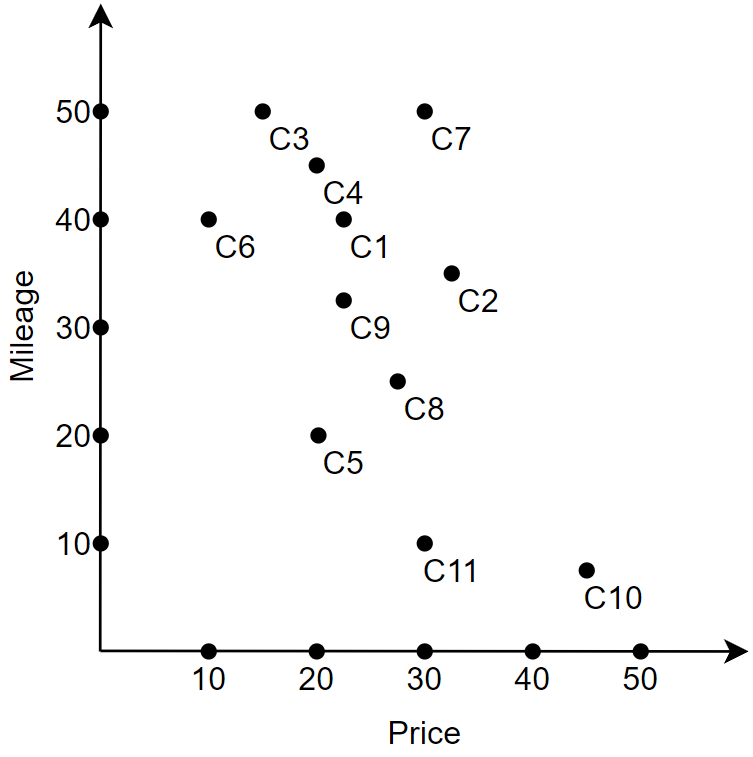
\includegraphics[width=0.25\linewidth]{images/ex1.png}
        \end{figure}
        If we choose $MaxP = 50,000$ and $MaxM = 80,000$, we have that a generic point $o$ is mapped with these formulas: 
        \[p_1(o) = 1 - \dfrac{o.Price}{MaxP} \:\:\:\:\:\: p_2(o) = 1 - \dfrac{o.Mileage}{MaxM}\]
        Graphically we have; 
        \begin{figure}[H]
            \centering
            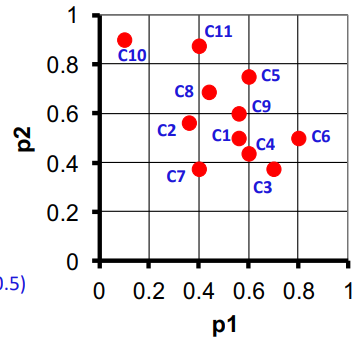
\includegraphics[width=0.3\linewidth]{images/ex2.png}
        \end{figure}
    \end{example}
    The most common scoring functions are: 
    \begin{itemize}
        \item Average (SUM), that weighs preferences equally
            \[\textnormal{SUM}(o) \equiv \textnormal{SUM}(p(o)) = p_1(o) + p_2(o) + \dots + p_m(o)\]
        \item Weighted sum (WSUM), that weighs the preferences differently
            \[\textnormal{WSUM}(o) \equiv \textnormal{WSUM}(p(o)) = w_1p_1(o) + w_2p_2(o) + \dots + w_mp_m(o)\]
        \item Minimum (MIN), that considers the worst partial score
            \[\textnormal{MIN}(o) \equiv \textnormal{MIN}(p(o)) = \min\{p_1(o),p_2(o),\dots, p_m(o)\}\]
        \item Maximum (MAX), that considers the best partial score
            \[\textnormal{MAX}(o) \equiv \textnormal{MAX}(p(o)) = \max\{p_1(o),p_2(o),\dots, p_m(o)\}\]       
    \end{itemize}
    Note that even with the minimum scoring function we always want to retrieve the $k$ objects with the highest global scores.

    It is possible to define e iso-score curves in the score space, which are set of points with the same global score. 
    \begin{example}
        In the previous graph we have that the iso-score curves for the maximum function are: 
        \begin{figure}[H]
            \centering
            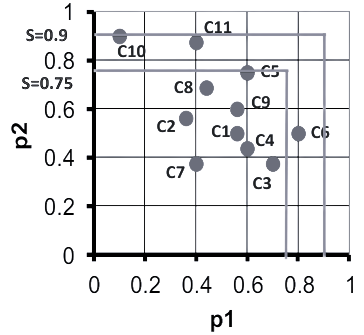
\includegraphics[width=0.3\linewidth]{images/iso.png}
        \end{figure}
        In the previous graph we have that the iso-score curves for the minimum function are: 
        \begin{figure}[H]
            \centering
            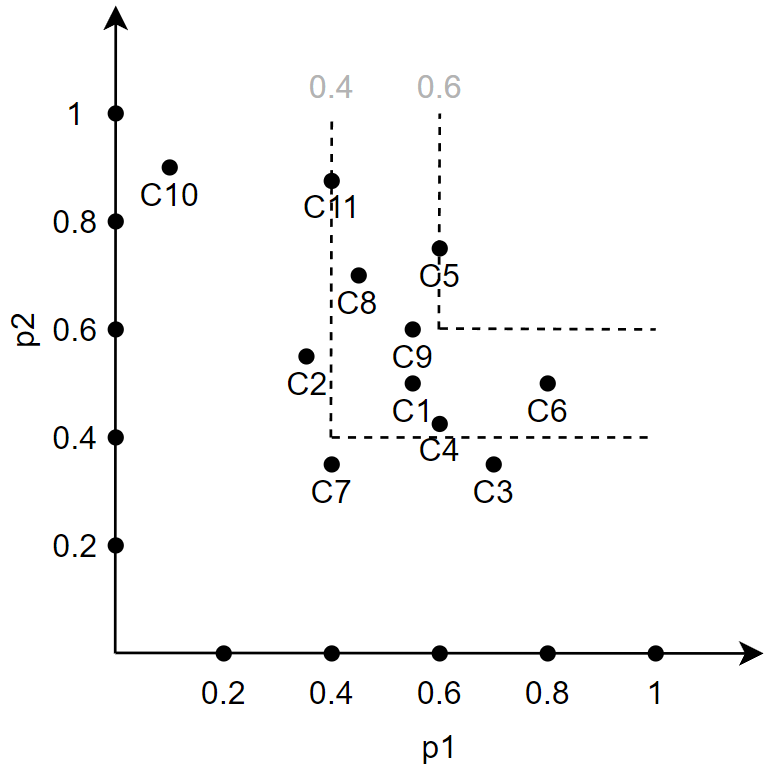
\includegraphics[width=0.3\linewidth]{images/isomin.png}
        \end{figure}
    \end{example}

    \subsection{B-zero algorithm}
    It is possible to efficiently compute the result of a top-k 1-1 join query using a maximum scoring function $S$ using the $B_0$ algorithm. The inputs
    of this algorithm are: an integer $k \geq 1$, and a ranked list $R_1,\dots,R_m$. The idea is: 
    \begin{enumerate}
        \item Make $k$ sorted accesses on each list and store objects and partial scores in a buffer $B$. 
        \item For each object in $B$, compute the MAX of its (available) partial scores.
        \item Return the $k$ objects with maximum score.
    \end{enumerate}
    This algorithm is instance-optimal. 
    \begin{example}
        Given the following reviews on two different sites: 
        \begin{table}[H]
            \centering
            \begin{tabular}{ccccc}
            \multicolumn{1}{l}{\textbf{EatWell}}     &                                     & $\:\:\:\:\:\:$                 & \multicolumn{1}{l}{\textbf{BreadAndWine}} &                                  \\ \cline{1-2} \cline{4-5} 
            \multicolumn{1}{|l}{\textbf{Name}}       & \multicolumn{1}{c|}{\textbf{Score}} & \multicolumn{1}{c|}{\textbf{}} & \multicolumn{1}{l}{\textbf{Name}}        & \multicolumn{1}{c|}{\textbf{Score}} \\ \cline{1-2} \cline{4-5} 
            \multicolumn{1}{|l}{The old mill}        & \multicolumn{1}{c|}{9.2}            & \multicolumn{1}{c|}{}          & \multicolumn{1}{l}{Da Gino}              & \multicolumn{1}{c|}{9.0}            \\
            \multicolumn{1}{|l}{The canteen}         & \multicolumn{1}{c|}{9.0}            & \multicolumn{1}{c|}{}          & \multicolumn{1}{l}{Cheers!}              & \multicolumn{1}{c|}{8.5}            \\  
            \multicolumn{1}{|l}{Cheers!}             & \multicolumn{1}{c|}{8.3}            & \multicolumn{1}{c|}{}          & \multicolumn{1}{l}{The old mill}         & \multicolumn{1}{c|}{7.5}            \\ 
            \multicolumn{1}{|l}{Da Gino}             & \multicolumn{1}{c|}{7.5}            & \multicolumn{1}{c|}{}          & \multicolumn{1}{l}{Chez Paul}            & \multicolumn{1}{c|}{7.5}            \\ 
            \multicolumn{1}{|l}{Let's eat!}          & \multicolumn{1}{c|}{6.4}            & \multicolumn{1}{c|}{}          & \multicolumn{1}{l}{The canteen}          & \multicolumn{1}{c|}{7.0}            \\ 
            \multicolumn{1}{|l}{Chez Paul}           & \multicolumn{1}{c|}{5.5}            & \multicolumn{1}{c|}{}          & \multicolumn{1}{l}{Los pollos hermanos}  & \multicolumn{1}{c|}{6.5}            \\ 
            \multicolumn{1}{|l}{Los pollos hermanos} & \multicolumn{1}{c|}{5.0}            & \multicolumn{1}{c|}{}          & \multicolumn{1}{l}{Let's eat!}           & \multicolumn{1}{c|}{6.0}            \\ \cline{1-2} \cline{4-5} 
            \end{tabular}
        \end{table}
        If we want to use the algorithm $B_0$ with $k=3$ we have to select the first three row from both tables (that are sorted), and by summing all the found values by identifier we
        obtain the final rank with the maximum value. In this case we obtain the following table: 
        \begin{table}[H]
            \centering
            \begin{tabular}{|lc|}
            \hline
            \textbf{Name} & \textbf{S} \\ \hline
            The old mill  & 9.2        \\ 
            Da Gino       & 9.0        \\ 
            The canteen   & 9.0        \\ 
            Cheers!       & 8.5        \\ \hline
            \end{tabular}
        \end{table}
    \end{example}

    \subsection{A-zero algorithm}
    The A-zero algorithm, also called Fagin's algorithm, works with every monotonic scoring function. The inputs
    of this algorithm are: an integer $k$, and a monotone function $S$ combining ranked lists $R_1,\dots,R_m$. The output is the top $k$ (object-score) tuples. 
    The idea of this algorithm is: 
    \begin{enumerate}
        \item Extract the same number of objects by sorted accesses in each list until there are at least $k$ objects in common. 
        \item For each extracted object, compute its overall score by making random accesses wherever needed. 
        \item Among these, output the $k$ objects with the best overall score. 
    \end{enumerate}
    The complexity of this algorithm is $O(N^{\frac{m-1}{m}}k^{\frac{1}{m}})$, that is sublinear in the number $N$ of objects. The 
    stopping criterion is independent of the scoring function, and it is not instance optimal. 
    \begin{example}
        Given the following hotel's review on different sites: 
        \begin{table}[H]
            \centering
            \begin{tabular}{|lc|c|lc|}
            \cline{1-2} \cline{4-5}
            \textbf{Name} & \textbf{Cheapness} & $\:\:\:\:\:\:$ & \textbf{Name} & \textbf{Rating} \\ \cline{1-2} \cline{4-5} 
            Ibis          & 0.92               &                & Crillon       & 0.9             \\ 
            Etap          & 0.91               &                & Novotel       & 0.9             \\  
            Novotel       & 0.85               &                & Sheraton      & 0.8             \\  
            Mercure       & 0.85               &                & Hilton        & 0.7             \\  
            Hilton        & 0.825              &                & Ibis          & 0.7             \\  
            Sheraton      & 0.8                &                & Ritz          & 0.7             \\  
            Crillon       & 0.75               &                & Lutetia       & 0.6             \\  
            $\dots$       & $\dots$            &                & $\dots$       & $\dots$         \\ \cline{1-2} \cline{4-5} 
            \end{tabular}
        \end{table}
        We decide to use the following scoring function: 
        \[0.5 \cdot cheapness+0.5 \cdot rating\]
        and $k=2$. We iterate on the rows until $k$ hotels are found in all columns. In this case we need to inspect $5$ column to find at
        least two hotels (we found: Ibis, Novotel and Hilton). Now we have to complete the score of the remaining incomplete hotels, so we make 
        random access to find the missing values. After summing completing the information about those hotels we can compute the final ranking 
        with the give score function, and we obtain: 
        \begin{table}[H]
            \centering
            \begin{tabular}{|lc|}
            \hline
            \textbf{Top $\boldsymbol{k}$} & \textbf{Score} \\ \hline
            Novotel                       & 0.875          \\ 
            Crillon                       & 0.825          \\ \hline
            \end{tabular}
        \end{table}
    \end{example}
    The main drawback of this algorithm is that it is dependent from the accesses, so the specificity of some scoring function is not exploited
    at all, and the memory requirements can become prohibitive. It is possible to make 
    some improvements, but only changing the stopping condition can really improve the complexity. 

    \subsection{Threshold algorithm}
    The inputs of the threshold algorithm are: an integer $k$, and a monotone function $S$ combining ranked lists $R_1,\dots,R_m$. 
    The output is the top $k$ (object, score) tuples. The idea of this algorithm is: 
    \begin{enumerate}
        \item Do sorted access in parallel in each list $R_i$. 
        \item For each object $o$, do random accesses in the other lists $R_j$, thus extracting score $s_j$. 
        \item Compute overall score $S(s_1, \dots, s_m)$. If the value is among the $k$ highest seen so far, and remember $o$. 
        \item Let $s_{L_i}$ be the last score seen under sorted access for $R_i$. 
        \item Define threshold $T=S(s_{L_1}, \dots, s_{L_m})$. 
        \item If the score of the $k$-th object is worse than $T$, go to step one. 
        \item Return the current top-$k$ objects. 
    \end{enumerate}
    The threshold algorithm is instance optimal among all algorithms that use random and sorted accesses, and the stopping criterion depends 
    on the function and not on the number of accesses. 
    \begin{example}
        Given the following hotel's review on different sites: 
        \begin{table}[H]
            \centering
            \begin{tabular}{|lc|c|lc|}
            \cline{1-2} \cline{4-5}
            \textbf{Name} & \textbf{Cheapness} & $\:\:\:\:\:\:$ & \textbf{Name} & \textbf{Rating} \\ \cline{1-2} \cline{4-5} 
            Ibis          & 0.92               &                & Crillon       & 0.9             \\ 
            Etap          & 0.91               &                & Novotel       & 0.9             \\ 
            Novotel       & 0.85               &                & Sheraton      & 0.8             \\ 
            Mercure       & 0.85               &                & Hilton        & 0.7             \\ 
            Hilton        & 0.825              &                & Ibis          & 0.7             \\ 
            Sheraton      & 0.8                &                & Ritz          & 0.7             \\ 
            Crillon       & 0.75               &                & Lutetia       & 0.6             \\ 
            $\dots$       & $\dots$            &                & $\dots$       & $\dots$         \\ \cline{1-2} \cline{4-5} 
            \end{tabular}
        \end{table}
        We decide to use the following scoring function: 
        \[0.5 \cdot cheapness+0.5 \cdot rating\]
        and $k=2$. We do a sorted access, and we put the hotels in the first row in the buffer with the mean value of both variables (the 
        second can be found with a random access). The threshold point is $(0.92,0.9)$ and has a value of $0.91$, found with the scoring 
        function. We continue to do this procedure, and we update the top $k$ hotels only if the found hotel has a better score of at least
        one of the hotels in the buffer (note that we keep in the buffer only the top $k$ hotels, while we delete the others). 
        We stop the iteration when the value of all the objects in the buffer is greater or equal to the threshold value. In this example this
        happens after three iteration. In fact, we have that the buffer contains the following values: 
        \begin{table}[H]
            \centering
            \begin{tabular}{|lc|}
            \hline
            \textbf{Top $\boldsymbol{k}$} & \textbf{Score} \\ \hline
            Novotel                       & 0.875          \\ 
            Crillon                       & 0.825          \\ \hline
            \end{tabular}
        \end{table}
        The threshold point has a value of $0.825$
    \end{example}
    In general, TA performs much better than FA, since it can adapt to the specific scoring function. In order to characterize the 
    performance of TA, we consider the middleware cost: 
    \[\textnormal{cost} = SA \cdot c_{SA} + RA \cdot c_{RA}\]
    where:
    \begin{itemize}
        \item $SA$ is the total number of sorted accesses.
        \item $RA$ is the total number of random accesses.
        \item $c_{SA}$ is the base cost of sorted accesses.
        \item $c_{RA}$ is the base cost of random accesses.
    \end{itemize}

    \subsection{No random access algorithm}
    The NRA returns the top-$k$ objects, but their scores might be uncertain. The idea at the base of this algorithm is to maintain, for each selected object
    $o$ a lower bound and an upper bound on its score. So, we need an unlimited buffer to 
    store the objects, sorted by decreasing lower bound values. This algorithm 
    stops when the new object upper bound is less or equal to the worst lower bound of the best objects. The inputs are: 
    an integer $k \geq 1$, a monotone function $S$ combining ranked lists $R_1, \dots, R_m$ and the output is the ranking
    without the score of the objects. The idea is the following: 
    \begin{enumerate}
        \item Make sorted access to each list. 
        \item Store in $B$ each retrieved object $o$ and maintain $S^{-}(o)$ and $S^{+}(o)$ and a threshold $\tau$. 
        \item Repeat from step one as long as:
            \[S^{-}(B[k]) < \max\{ \max\{S^{+}(B[i]), i > k\}, S(\tau) \}\]
    \end{enumerate}
    \begin{example}
        Given the following tables based on three different criterions: 
        \begin{table}[H]
            \centering
            \begin{tabular}{cccccccc}
            \multicolumn{1}{l}{$R_1$}                 & \multicolumn{1}{l}{}                & \multicolumn{1}{l}{$\:\:\:\:\:\:$} & \multicolumn{1}{l}{$R_2$}                & \multicolumn{1}{l}{}                & \multicolumn{1}{l}{$\:\:\:\:\:\:$} & \multicolumn{1}{l}{$R_3$}                & \multicolumn{1}{l}{}                \\ \cline{1-2} \cline{4-5} \cline{7-8} 
            \multicolumn{1}{|c}{\textbf{ID}} & \multicolumn{1}{c|}{\textbf{Score}} & \multicolumn{1}{c|}{\textbf{}}     & \multicolumn{1}{c}{\textbf{ID}} & \multicolumn{1}{c|}{\textbf{Score}} & \multicolumn{1}{c|}{\textbf{}}     & \multicolumn{1}{c}{\textbf{ID}} & \multicolumn{1}{c|}{\textbf{Score}} \\ \cline{1-2} \cline{4-5} \cline{7-8} 
            \multicolumn{1}{|c}{$o_1$}               & \multicolumn{1}{c|}{1.0}            & \multicolumn{1}{c|}{}              & \multicolumn{1}{c}{$o_2$}               & \multicolumn{1}{c|}{0.8}            & \multicolumn{1}{c|}{}              & \multicolumn{1}{c}{$o_7$}               & \multicolumn{1}{c|}{0.6}            \\  
            \multicolumn{1}{|c}{$o_7$}               & \multicolumn{1}{c|}{0.9}            & \multicolumn{1}{c|}{}              & \multicolumn{1}{c}{$o_3$}               & \multicolumn{1}{c|}{0.75}           & \multicolumn{1}{c|}{}              & \multicolumn{1}{c}{$o_2$}               & \multicolumn{1}{c|}{0.6}            \\  
            \multicolumn{1}{|c}{$o_2$}               & \multicolumn{1}{c|}{0.7}            & \multicolumn{1}{c|}{}              & \multicolumn{1}{c}{$o_4$}               & \multicolumn{1}{c|}{0.5}            & \multicolumn{1}{c|}{}              & \multicolumn{1}{c}{$o_3$}               & \multicolumn{1}{c|}{0.5}            \\  
            \multicolumn{1}{|c}{$o_6$}               & \multicolumn{1}{c|}{0.2}            & \multicolumn{1}{c|}{}              & \multicolumn{1}{c}{$o_1$}               & \multicolumn{1}{c|}{0.4}            & \multicolumn{1}{c|}{}              & \multicolumn{1}{c}{$o_5$}               & \multicolumn{1}{c|}{0.1}            \\  
            \multicolumn{1}{|c}{$\dots$}             & \multicolumn{1}{c|}{$\dots$}        & \multicolumn{1}{c|}{}              & \multicolumn{1}{c}{$\dots$}             & \multicolumn{1}{c|}{$\dots$}        & \multicolumn{1}{c|}{}              & \multicolumn{1}{c}{$\dots$}             & \multicolumn{1}{c|}{$\dots$}        \\ \cline{1-2} \cline{4-5} \cline{7-8} 
            \end{tabular}
        \end{table}
        We decide to use SUM as score function, and $k=2$. For the first iteration we add to the buffer the  objects in the first row with a lower bound corresponding to 
        the sum of the score of each object and the upper bound corresponding to the sum of all the object in the row. The threshold is the sum of all the scores of the row: 
        \begin{table}[H]
            \centering
            \begin{tabular}{|ccc|}
            \hline
            \textbf{Identifier} & \textbf{Lower bound} & \textbf{Upper bound} \\ \hline
            $o_1$               & 1.0                  & 2.4                  \\ 
            $o_2$               & 0.8                  & 2.4                  \\ 
            $o_7$               & 0.6                  & 2.4                  \\ \hline
            \end{tabular}
        \end{table}
        The threshold has a value of $2.4$, and so we have that:
        \[0.8<\max\{2.4,2.4\}\]
        Since that the inequality is verified we have to do another iteration, that creates the following table: 
        \begin{table}[H]
            \centering
            \begin{tabular}{|ccc|}
            \hline
            \textbf{Identifier} & \textbf{Lower bound} & \textbf{Upper bound} \\ \hline
            $o_7$               & 1.5                  & 2.25                 \\ 
            $o_2$               & 1.4                  & 2.3                  \\ 
            $o_1$               & 1.0                  & 2.35                 \\ 
            $o_3$               & 0.75                 & 2.25                 \\ \hline
            \end{tabular}
        \end{table}
        The threshold has a value of $2.25$, and so we have that:
        \[1.4<\max\{2.35,2.25\}\]
        Since that the inequality is verified we have to do another iteration, that creates the following table: 
        \begin{table}[H]
            \centering
            \begin{tabular}{|ccc|}
            \hline
            \textbf{Identifier} & \textbf{Lower bound} & \textbf{Upper bound} \\ \hline
            $o_2$               & 2.1                  & 2.1                  \\ 
            $o_7$               & 1.5                  & 2.0                  \\ 
            $o_3$               & 1.25                 & 1.95                 \\
            $o_1$               & 1.0                  & 2.0                  \\ 
            $o_4$               & 0.5                  & 1.7                  \\ \hline
            \end{tabular}
        \end{table}
        The threshold has a value of $1.7$, and so we have that:
        \[1.5<\max\{2.0,1.7\}\]
        Since that the inequality is verified we have to do another iteration, that creates the following table: 
        \begin{table}[H]
            \centering
            \begin{tabular}{|ccc|}
            \hline
            \textbf{Identifier} & \textbf{Lower bound} & \textbf{Upper bound} \\ \hline
            $o_2$               & 2.1                  & 2.1                  \\ 
            $o_7$               & 1.5                  & 1.9                  \\ 
            $o_1$               & 1.4                  & 1.5                  \\ 
            $o_3$               & 1.25                 & 1.45                 \\ 
            $o_4$               & 0.5                  & 0.8                  \\ 
            $o_6$               & 0.2                  & 0.7                  \\ 
            $o_5$               & 0.1                  & 0.7                  \\ \hline
            \end{tabular}
        \end{table}
        The threshold has a value of $1.7$, and so we have that:
        \[1.5<\max\{1.5,0.7\}\]
        Since that the inequality is not verified the algorithm return the first two elements in the table. 
    \end{example}
    NRA is instance optimal among all algorithms that do not make random accesses.
    
    \subsection{Summary}
    \begin{table}[H]
        \centering
        \resizebox{\columnwidth}{!}{%
        \begin{tabular}{l|ccc}
        \multicolumn{1}{c|}{\textbf{Algorithm}} & \textbf{Scoring function} & \textbf{Data access} & \textbf{Notes}                       \\ \hline
        $B_0$                                   & MAX                       & sorted               & instance-optimal                     \\
        FA                                      & monotone                  & sorted and random    & cost independent of scoring function \\
        TA                                      & monotone                  & sorted and random    & instance-optimal                     \\
        NRA                                     & monotone                  & sorted               & instance-optimal, uncertain         
        \end{tabular}%
        }
    \end{table}

    The main aspects of the ranking queries are: 
    \begin{itemize}
        \item They are very effective identifying the best objects with respect to a specific scoring function. 
        \item They have excellent control of the cardinality of the result. 
        \item The computation is very efficient. 
        \item It is easy to express the relative importance of attributes. 
        \item For a user, it is difficult to specify a scoring function. 
    \end{itemize}

    \section{Skyline queries}
    The objective of the skyline queries is to find good objects according to several perspectives, that are based on the notion of dominance. 
    \begin{definition}
        A tuple $t$ \emph{dominates} a tuple $s$ ($t \prec s$) if and only if $t$ in nowhere worse than $s$: 
        \[\forall i, 1 \leq i \leq m \rightarrow t[A_i] \leq s[A_i]\] 
        and better at least once: 
        \[\exists j, 1 \leq j \leq m \land t[A_j] < s[A_j]\]


        The \emph{skyline} of a relation is the set of its non dominated tuples
    \end{definition}
    The convention on the skyline queries is that lower values are better than higher values. A tuple $t$ is in the skyline if
    and only if  it is the top-$1$ result with respect to at least one monotone scoring function. This means that the skyline is the set of potentially optimal tuples. 
    Note that there is no scoring function that returns the same points that are in the skyline. A possible non-standard syntax for the 
    skyline queries is the following: 
    \begin{lstlisting}[style=SQL]
SELECT <attributes>
FROM R1,R2,...,Rn
WHERE <conditions>
GROUP BY <conditions>
HAVING <conditions>
SKYLINE OF [DISTINCT] d1[MIN|MAX|DIFF], ..., dm[MIN|MAX|DIFF]
ORDER BY <conditions>
    \end{lstlisting}
    This query can be easily translated into a standard query, but the result is too slow and cannot be used in practice. 

    \subsection{Block nested loop algorithm}
    The input of the block nested loop algorithm is a dataset $D$ of multidimensional points, and the output is the skyline of $D$.
    \begin{algorithm}[H]
        \caption{Block nested loop algorithm}
            \begin{algorithmic}[1]
                \State $W \leftarrow \varnothing$
                \For {every point $p$ in $D$}
                    \If {$p$ not dominated by any point in $W$}
                        \State remove from $W$ the points dominated by $p$
                        \State add $p$ to $W$
                    \EndIf
                \EndFor
                \State \Return $W$
            \end{algorithmic}
    \end{algorithm}
    The complexity is $O(n^2)$, where $n=\left\lvert D \right\rvert $. The complexity of this algorithm is very inefficient for large datasets. 

    \subsection{Sort filter skyline algorithm}
    The input of the sort filter skyline algorithm is a dataset $D$ of multidimensional points, and the output is the skyline of $D$.
    \begin{algorithm}[H]
        \caption{Sort filter skyline algorithm}
            \begin{algorithmic}[1]
                \State $S \leftarrow D$
                \State $W \leftarrow \varnothing$
                \For {every point $p$ in $S$}
                    \If {$p$ not dominated by any point in $W$}
                        \State add $p$ to $W$
                    \EndIf
                \EndFor
                \State \Return $W$
            \end{algorithmic}
    \end{algorithm}
    Where $S$ is the list of sorted point in $D$ by a monotone function. The initial sorting is useful for large datasets, thus this algorithm performs much better than the
    previous one, although the complexity is still $O(n^2)$. 
    \begin{example}
        Given the following unordered dataset: 
        \begin{table}[H]
            \centering
            \begin{tabular}{lcc}
            \textbf{Name}                 & \textbf{Cost} & \textbf{Complaints} \\ \hline
            \multicolumn{1}{l|}{Crillon}  & 0.25  & 0.1        \\
            \multicolumn{1}{l|}{Ibis}     & 0.08  & 0.3        \\
            \multicolumn{1}{l|}{Hilton}   & 0.175 & 0.3        \\
            \multicolumn{1}{l|}{Sheraton} & 0.2   & 0.2        \\
            \multicolumn{1}{l|}{Novotel}  & 0.15  & 0.1       
            \end{tabular}
        \end{table}
        We decide to order them by the sum of cost and complaints, and the resulting dataset is: 
        \begin{table}[H]
            \centering
            \begin{tabular}{lcc}
            \textbf{Name}                 & \textbf{Cost} & \textbf{Complaints} \\ \hline
            \multicolumn{1}{l|}{Novotel}  & 0.15          & 0.1                 \\
            \multicolumn{1}{l|}{Crillon}  & 0.25          & 0.1                 \\
            \multicolumn{1}{l|}{Ibis}     & 0.08          & 0.3                 \\
            \multicolumn{1}{l|}{Sheraton} & 0.2           & 0.2                 \\
            \multicolumn{1}{l|}{Hilton}   & 0.175         & 0.3                
            \end{tabular}
        \end{table}
        The algorithm adds Novotel to the window, and the other hotel that is not dominated by Novotel is Ibis, so the skyline is composed by Novotel and Ibis. 
    \end{example}

    \subsection{Summary}
    The main aspects of the skyline queries are: 
    \begin{itemize}
        \item They are effective in identifying potentially interesting objects if nothing is known about the preferences of a user. 
        \item They are very simple to use. 
        \item They return too many objects. 
        \item The computation is not so efficient. 
        \item They are agnostic with respect to user preferences
    \end{itemize}
    It is possible to extend the skyline queries adding the constraint of set of tuples dominated by less than $k$ tuples. This method is called $k$-skyband.

    \section{Comparison between ranking and skyline}
    \begin{table}[H]
        \centering
        \begin{tabular}{l|cc|}
        \cline{2-3}
                                                         & \textbf{Ranking queries} & \textbf{Skyline queries} \\ \hline
        \multicolumn{1}{|l|}{Simplicity}                 & No              & Yes             \\
        \multicolumn{1}{|l|}{Only interesting results}   & No              & Yes             \\
        \multicolumn{1}{|l|}{Control of cardinality}     & Yes             & No              \\
        \multicolumn{1}{|l|}{Trade-off among attributes} & Yes             & No              \\ \hline
        \end{tabular}
    \end{table}

\newpage 

\chapter{Architectures and JPA}
    \section{Introduction}
    \begin{definition}
        The \emph{architecture} is the union of hardware, software, and network resources. 
    \end{definition}
    The actual architectures are: 
    \begin{itemize}
        \item Distributed web-based and mobile. 
        \item Service oriented. 
        \item Cloud and virtualized. 
        \item Application service provisioning. 
    \end{itemize}
    \begin{chronology}[10]{1959}{2010}{\columnwidth}
        \event[1960]{1969}{One-tier architectures}
        \event[1970]{1980}{Client-Server architectures}
        \event{1980}{Distributed architectures based on RPC}
        \event{1990}{Object oriented distributed architectures}
        \event[1995]{2000}{Internet and Web-based architectures}   
    \end{chronology}

    \section{Client-server architecture}
    \begin{figure}[H]
        \centering
        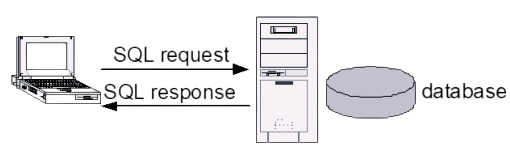
\includegraphics[width=0.4\linewidth]{images/cs.png}
        \caption{Client-server architecture}
    \end{figure}
    The hardware used by this the client-server architecture is: 
    \begin{itemize}
        \item Server for data management. 
        \item Client for presentation layout. 
    \end{itemize}
    The software used by this type of architecture is: 
    \begin{itemize}
        \item Client software sends requests to the server by means of SQL queries. The software in the client contains both business and presentation logic. 
        \item Server software processes the query and responds sending the result set back to the client. The software in the server deals with data. 
    \end{itemize}
    The network topology is based on a local are network with one or more servers and $N$ clients. 

    \section{Three-tier architecture}
    \begin{figure}[H]
        \centering
        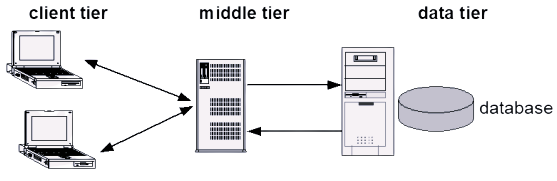
\includegraphics[width=0.5\linewidth]{images/tt.png}
        \caption{Three-tier architecture}
    \end{figure}
    The hardware used by the three-tier architecture is: 
    \begin{itemize}
        \item Server for data management. 
        \item Client for presentation layout. 
        \item Middle tier to achieve a better separation between the client and the server. 
    \end{itemize}
    This architecture has several variants, depending on the software features of the middle tier. 
    
    \subsection{Web pure HTML three-tier architecture}
    \begin{figure}[H]
        \centering
        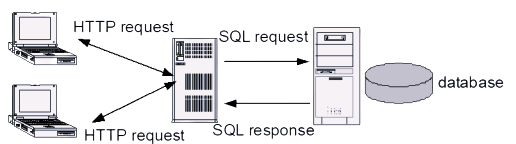
\includegraphics[width=0.5\linewidth]{images/ttph.png}
        \caption{Web pure HTML three-tier architecture}
    \end{figure}
    In the pure HTML architecture the client is a standard web browser, and it has to cope with the presentation layout only (thin client). The middle tier: 
    \begin{itemize}
        \item Includes a Web server that exploits HTTP.
        \item Hosts the business logic for dynamically generating content from the raw data of the data tier. 
        \item Deals with the presentation layout. 
    \end{itemize}

    \subsection{Rich internet applications}
    \begin{figure}[H]
        \centering
        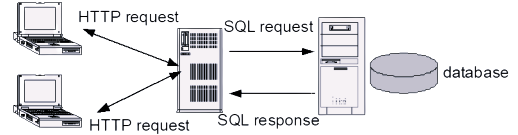
\includegraphics[width=0.5\linewidth]{images/ttria.png}
        \caption{Rich internet applications three-tier architecture}
    \end{figure}
    The rich internet application architecture is the fusion of web and desktop applications (with JavaScript). 
    In this case the client is called fat because it has standard communication protocol (HTTP, Web Socket), language (ECMAScript) and API (DOM, HTML5). 
    The features of this architecture are: 
    \begin{itemize}
        \item New interface event types, also specific to touch and mobile apps.
        \item Asynchronous interaction (AJAX).
        \item Client-side persistent data.
        \item Offline applications.
        \item Native multimedia and 3D support.
    \end{itemize}

    \section{Java enterprise edition}
    Java enterprise edition is a platform aimed at the development, release and maintenance of three-tier web applications.
    \begin{figure}[H]
        \centering
        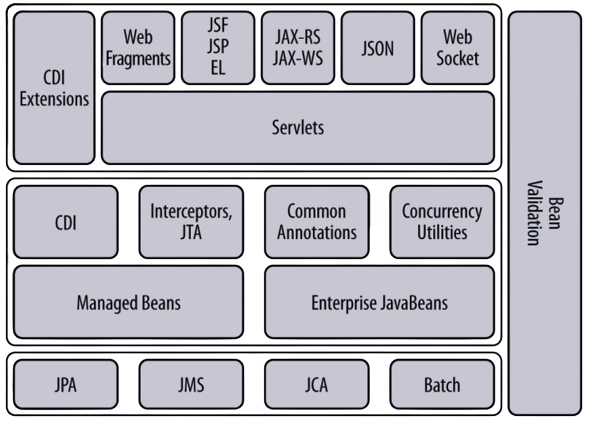
\includegraphics[width=0.5\linewidth]{images/jee.png}
        \caption{Jakarta EE stack}
    \end{figure}
    The main elements of this platform are: 
    \begin{itemize}
        \item JDBC: this API was the first industry standard for database independent connectivity between Java and the database. Thanks to this API we can:
            establish a connection with a database, send SQL statements, and process the results. 
        \item Servlet, that are the Java technology for the presentation tier in web application. The servlets: 
            offer a component-based, platform independent method for building web-based applications, have access to other Java APIs to access enterprise databasesa 
            and are executed within a container for concurrency control and lifecycle management. 
        \item Jakarta Enterprise Beans: it is the technology used in the server. They enable the development of distributed, transactional, secure and portable applications. 
            EJB components can be used by the web front-end to interact with the business functions and data access services. 
        \item Java Persistence API: it is the specification of an interface for mapping relational data to object oriented data in Java. 
            It comprises: the API implementation package javax.persistence, the Java compatible query language Java Persistence Query Language, and the specification of the metadata for defining object
            relational mappings. 
        \item Java Transaction API: it is an API for managing transactions in Java. It allows a component to start, commit and rollback transactions in a resource agnostic way. 
            With this technology, Java components can manage multiple resources in a single transaction with a unique interaction model.
    \end{itemize}
    \begin{example}
        To extract data from a database using JPA we use: 
        \begin{lstlisting}[style=Java]
public List<Mission> findMissionsByUser(int userId) {
    Reporter reporter = em.find(Reporter.class, userId);
    List<Mission> missions = reporter.getMissions();
    return missions;
}
        \end{lstlisting}
        To insert data in a database using JPA we use: 
        \begin{lstlisting}[style=Java]
public void createMission(Date startDate, int days, String destination, String description, int reporterId) {
    Reporter reporter = em.find(Reporter.class, reporterId);
    Mission mission = new Mission(startDate, days, destination, description, reporter);
    reporter.addMission(mission);
    em.persist(reporter);
}        
        \end{lstlisting}
        To modify data in a database using JPA we use: 
        \begin{lstlisting}[style=Java]
public void reportMission(int missionId, MissionStatus missionStatus) {
    Mission mission = em.find(Mission.class, missionId);
    mission.setStatus(MissionStatus.REPORTED);
}
        \end{lstlisting}
    \end{example}






    \section{JPA: Object Relational Mapping}
        The technique of bridging the gap between the object model and the relational model is known as object-relational mapping. 
        \begin{definition}
            The challenge of mapping one model to the other lies in the concepts in one model for which there is no logical equivalent in the other is called 
            \emph{impedance mismatch}.
        \end{definition}
        The automatic transformation of a model into another in managed by an element called mediator. The main differences between the object-oriented model and the 
        relational one are the followings: 
        \begin{table}[H]
            \centering
            \begin{tabular}{cc}
            \hline
            \textbf{Object-oriented model}     & \textbf{Relational model}   \\ \hline
            Objects, classes                   & Tables, rows                \\
            Attributes, properties             & Columns                     \\
            Identity (physical memory address) & Primary key                 \\
            Reference to other entity          & Foreign key                 \\
            Inheritance/Polymorphism           & Not supported               \\
            Methods                            & Stored procedures, triggers \\
            Code is portable                   & Not necessarily portable    \\ \hline
            \end{tabular}
        \end{table}
        The Java Persistence API bridges the gap between object-oriented domain models and relational database systems by using a Plain Old Java Object, that is a 
        persistence model for object-relational mapping. 

        The main features of the Java Persistence API are: 
        \begin{itemize}
            \item POJO Persistence: there is nothing special about the objects being persisted, any existing non-final object with a default constructor can be persisted.
            \item Non-intrusiveness: the persistence API exists as a separate layer from the persistent objects.
            \item Object queries: a powerful query framework offers the ability to query across entities and their relationships without having to use concrete foreign keys or database columns.
        \end{itemize}

        \begin{definition}
            The \emph{entity} is a class (Java bean) representing a collection of persistent objects mapped onto a relational table. 

            The \emph{persistence unit} is the set of all classes that are persistently mapped to one database (analogous to the notion of db schema). 

            The \emph{persistence context} is the set of all managed objects of the entities defined in the persistence unit (analogous to the notion of db instance). 

            The \emph{managed entity} is an entity part of a persistence context for which the changes of the state are tracked. 

            The \emph{entity manager} is the interface for interacting with a persistence context. 
            
            The \emph{client} is a component that can interact with a persistence context, indirectly through an entity manager.
        \end{definition}
        The entities are accessed through the entity manager interface of the Java Persistence API. 
        \begin{figure}[H]
            \centering
            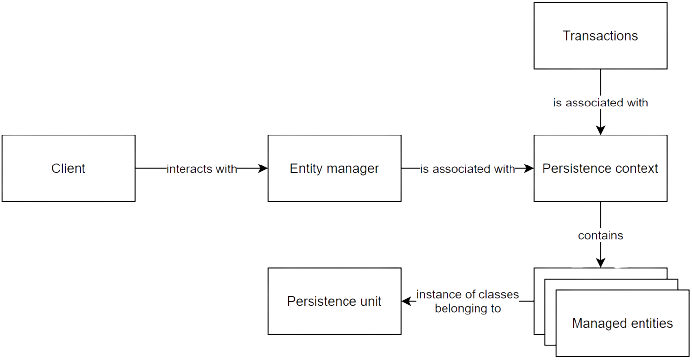
\includegraphics[width=0.9\linewidth]{images/jpa.png}
            \caption{Structure of the Java Persistence API}
        \end{figure}
        The entity manager exposes all the operations needed to synchronize the managed entities in the persistence context to the database to:
        \begin{itemize}
            \item Persist an entity instance in the database.
                \begin{lstlisting}[style=Java]
public void persist(Object entity);
                \end{lstlisting}
            \item Find an entity instance by its primary key.
                \begin{lstlisting}[style=Java]
public <T> T find(Class<T> entityClass, Object primaryKey); 
                \end{lstlisting}
            \item Remove an entity instance from the database.
                \begin{lstlisting}[style=Java]
public void remove(Object entity); 
                \end{lstlisting}
            \item Reset the entity instance from the database.
                \begin{lstlisting}[style=Java]
public void refresh(Object entity); 
                \end{lstlisting}
            \item Write the state of entities to the database immediately.
                \begin{lstlisting}[style=Java]
public void flush();
                \end{lstlisting}
        \end{itemize}
        An entity is a Java Bean that gets associated to a tuple in a database. The persistent counterpart of an entity has a life longer than that of the application. 
        The entity class must be associated with the database table it represents. An entity can enter a managed state, where all the modifications to the object's state
        are tracked and automatically synchronized to the database. The entities have the following properties: identification (primary key), nesting, relationship, 
        referential integrity (foreign key), and inheritance. The entities must respect the following requirements:
        \begin{itemize}
            \item Must have a public or protected constructor with no arguments. 
            \item Must not be final.
            \item No method or persistent instance variables may be final.
            \item Serializable interface must be implemented if you pass the entity by value.
        \end{itemize}
        
        In the database, objects and tuples have an identity (primary key), so an entity assumes the identity of the persistent data it is associated to. The primary key can be 
        either simple or composite. To identify a primary key we use the @Id annotation, for the composite keys we use @EmbeddedId and @IdClass annotations. 
        
        Sometimes, applications do not want to explicitly manage uniqueness of data values. In this case the persistence provider can automatically generate an identifier 
        for every entity instance of a given type. This persistence provider's feature is called identifier generation and is specified by the @GeneratedValue annotation. 
        Applications can choose one of four different ID generation strategy: 
        \begin{enumerate}
            \item Auto. 
            \item Table: identifiers are generated according to a generator table.
            \item Sequence: the identifiers are generated with sequences. 
            \item Identity: the identifiers are generated with primary keys identity columns. 
        \end{enumerate}
        \begin{example}
            An identifier can be generated as follows: 
            \begin{lstlisting}[style=Java]
@Entity
public class Mission implements Serializable {
    @Id
    @GeneratedValue(strategy = GenerationType.IDENTITY)
    private int id;
    private String city;
}
            \end{lstlisting}
        \end{example}
        The attributes can be qualified with properties that direct the mapping between POJO and relational tables, such as: 
        \begin{itemize}
            \item Large objects.
            \item Enumerated types: Java enumerations and strings. 
            \item Temporal types.
        \end{itemize}
        The fetch policy can be lazy (retrieve item when needed) or eager (retrieve item as soon as possible). The first policy is used mainly for large objects. 
        \begin{example}
            The qualifiers can be used as follows: 
            \begin{lstlisting}[style=Java]
@Entity
public class Mission implements Serializable {
    @Id
    @GeneratedValue(strategy = GenerationType.IDENTITY)
    private int id;
    @Temporal(TemporalType.DATE)
    private Date date;
    private MissionStatus status;
    @Basic(fetch=FetchType.LAZY)
    @LOB
    private byte[] photo;
}
            \end{lstlisting}
        \end{example}
        By default, entities are mapped to tables with the same name and their fields to columns with the same names, but it is possible to use some annotations 
        to change this behavior. If the entity must be not persistent, we have to denote it with @Transient annotation. 
        \begin{example}
            The mapping can be redefined as follows: 
            \begin{lstlisting}[style=Java]
@Entity @Table(name="T_BOOKS")
public class Book {
    @Column(name="BOOK_TITLE", nullable=false)
    private String title;
    private CoverType coverType;
    private Date publicationDate;
    @Transient
    private BigDecimal discount;
}
            \end{lstlisting}
        \end{example}

        \subsection{Mapping}
        The relationships in any object model has four characteristics:
        \begin{itemize}
            \item Directionality: each of the two entities may have an attribute that enables access to the other one. If two entities are related with each other we have 
                a bidirectional relationship; otherwise we have a unidirectional relationship. It is possible to have one or more references. 
            \item Role: each entity in the relationship is said to play a role with respect to one direction of access. The entities are classified in source and target,
                based on the direction of the relationship. 
            \item Cardinality: the number of entity instances that exist on each side of the relationship. There are four possibilities: 
                \begin{itemize}
                    \item Many-to-one: many source entities, one target entity.
                    \item One-to-many: one source entity, many target entities.
                    \item One-to-one: one source entity, one target entity.
                    \item Many-to-many: many source entities, many target entities.
                \end{itemize}
            \item Ownership: one of the two entity in the relationship is said to own the relationship. In the database, relationships are implemented by a foreign key 
                column (called join column in JPA) that refers to the key of the referenced table. The entities that have  a foreign key column is called the owner of 
                the relationship and its side is called the owning side
        \end{itemize}

        \subsection{One-to-many relationship}
        The one-to-many bidirectional relationship is defined with mappedBy and @ManyToOne, @OneToMany annotations, where: 
        \begin{itemize}
            \item @ManyToOne annotation to the entity that participates with multiple instances. The entity that contains this annotation is the owner of the relationship. 
            \item @JoinColumn annotation to specify the foreign key column of underlying table. 
        \end{itemize}
        \begin{example}
            First part of the definition of a one-to-many bidirectional mapping. 
            \begin{lstlisting}[style=Java]
@Entity
public class Employee {
    @Id private int id;
    @ManyToOne
    @JoinColumn(name="dept_fk")
    private Department dept;
}
            \end{lstlisting}
        \end{example}
        To achieve bi-directionality, the one-to-many mapping direction must be specified too. This is done by including a @OneToMany annotation in the entity that 
        participates with one instance. The @OneToMany annotation is placed on a collection data member and comprises a mappedBy element to indicate the property that 
        implements the inverse of the relationship.
        \begin{example}
            Second part of the definition of a one-to-many bidirectional mapping. 
            \begin{lstlisting}[style=Java]
@Entity
public class Department {
    @Id private int id;
    @OneToMany(mappedBy="dept")
    private Collection<Employee> employees;
}
            \end{lstlisting}
        \end{example}
        Sometimes applications require the access to relationships only along one direction, and in this case the bidirectional mapping is not necessary. 
        
        \subsection{Many-to-one relationship}
        The many-to-one relationship is defined in the same way as the one-to-many, but the source and the target are switched in the definition. 

        \subsection{One-to-one relationship}
        To define a one-to-one relationship in JPA it is possible to choose between two different alternatives: 
        \begin{itemize}
            \item We map the relationship as in the bidirectional case and use only the one-to-many direction. 
            \item We do not map the collection attribute in the entity that participates with one instance and use a query instead to retrieve the correlated instances, 
                relying on the inverse (many-to-one) relationship direction mapping.
        \end{itemize}
        The difference between @joincolumn and mappedby is the following: 
        \begin{itemize}
            \item The annotation @JoinColumn indicates the foreign key column that implements the relationship in the database; such annotation is normally inserted in 
                the entity owner of the relationship. Used to drive the generation of the SQL code to extract the correlated instances.
            \item The mappedBy attribute indicates that this side is the inverse of the relationship, and the owner resides in the other related entity. Used to 
                specify bidirectional relationships. In absence of the mappedBy parameter the default JPA mapping uses a bridge table.
        \end{itemize}
        In a one-to-one mapping the owner can be either entity, depending on the database design. A one-to-one mapping is defined by annotating the owner entity 
        with the @OneToOne annotation.
        \begin{example}
            First part of the definition of a one-to-one mapping. 
            \begin{lstlisting}[style=Java]
@Entity
public class Employee {
    @Id private int id;
    @OneToOne
    private ParkingSpace parkingSpace;
}
            \end{lstlisting}
        \end{example}
        If the one-to-one mapping is bidirectional, the inverse side of the relationship needs to be specified too. In the non-owner entity we need both @OneToOne annotation 
        and the mappedBy element (used to JPA to understand where to put the foreign key).
        \begin{example}
        Second part of the definition of a one-to-one mapping. 
            \begin{lstlisting}[style=Java]
@Entity
public class ParkingSpace {
    @Id private int id;
    @OneToOne(mappedBy="parkingSpace")
    private Employee employee;
}
            \end{lstlisting}
        \end{example}

    \subsection{Many-to-many relationship}
        In a many-to-many mapping there is no foreign key column, but there is a join table. Therefore, we can arbitrarily specify as owner either entity.
    \begin{example}
        First part of the definition of a many-to-many mapping. 
            \begin{lstlisting}[style=Java]
@Entity
public class Employee {
    @Id private int id;
    @ManyToMany
    private Collection<Project> projects;
}
            \end{lstlisting}
        \end{example}
        If the many-to-many mapping is bidirectional, the inverse side of the relationship needs to be specified too. In the non-owner entity we need both @OneToOne 
        annotation and the mappedBy element.
        \begin{example}
        First part of the definition of a many-to-many mapping. 
            \begin{lstlisting}[style=Java]
@Entity
public class Project {
    @Id private int id;
    @ManyToMany(mappedBy="projects")
    private Collection<Employee> employees;
}
            \end{lstlisting}
        \end{example}
        The logical model of a many-to-many relationship requires a bridge table (join table in JPA). 
        \begin{example}
            The non-default mapping of the entity to the bridge table is specified via annotation. 
            \begin{lstlisting}[style=Java]
@Entity
public class Employee {
    @Id private long id;
    private String name;
    @ManyToMany
    @JoinTable(name="EMP_PROJ",
                joinColumns=@JoinColumn(name="EMP_ID"),
                inverseJoinColumns=@JoinColumn(name="PROJ_ID"))
    private Collection<Project> projects;
}
            \end{lstlisting}
        \end{example}
    
    \subsection{Relationship fetch mode}
    When the fetch mode is not specified, by default:
    \begin{itemize}
        \item A single-valued relationship is fetched eagerly. 
        \item Collection-valued relationships are loaded lazily
    \end{itemize}
    In case of bidirectional relationships, the fetch mode might be lazy on one side but eager on the other. Note that the best practice is to consider lazy loading 
    as the most appropriate mode for all relationships because if an entity as many single-valued relationships that are not all used by applications, the eager mode may 
    incur performance penalties. 
    \begin{example}
        The annotation used to define the lazy loading.
        \begin{lstlisting}[style=Java]
@Entity
public class Employee {
    @Id private int id;
    @OneToOne(fetch=FetchType.LAZY)
    private ParkingSpace parkingSpace;
}
        \end{lstlisting}
    \end{example}
    The directive to lazily fetch an attribute is meant only to be a hint to the persistence provider, that can still use an eager policy. The other way round is not true: 
    the eager policy cannot be replaced with a lazy one by the provider. 

    \subsection{Cascading operations}
    By default, every entity manager operation will not cascade to other entities that have a relationship with the entity that is being operated on. In some cases we want 
    to have the propagation of the changes to the entities in relationship with the modified one. It is possible to do so by activating manual cascading. 
    \begin{example}
        Activation of manual cascading: 
        \begin{lstlisting}[style=Java]
Employee emp = new Employee();
Address addr = new Address();
emp.setAddress(addr);
em.persist(addr);
em.persist(emp);
        \end{lstlisting}
        With this mode activated, when the entity manager adds the Employee instance to the persistence context, it navigates the address relationship looking for a 
        new Address entity to manage as well. The Address instance must be set on the Employee instance before invoking persist() on the employee object. If an Address 
        instance has been set on the Employee instance and not persisted explicitly or implicitly via cascading, an error occurs.
    \end{example}
    The cascade attribute is used to define when operations should be automatically cascaded across relationships. It accepts several values: 
    \begin{itemize}
        \item Persist. 
        \item Refresh. 
        \item Remove.
        \item Merge.
        \item Detach.
    \end{itemize}
    If we want to use all the previous operations we can use the operator "all". 
    \begin{example}
        Activation of manual cascading of type persist: 
        \begin{lstlisting}[style=Java]
@Entity
public class Employee {
    @ManyToOne(cascade=CascadeType.PERSIST)
    Address address;
}
        \end{lstlisting}
    \end{example}
    The cascade settings are unidirectional, so they must be set on both side if we want a bidirectional behavior. 

    JPA also supports an additional remove cascading called "orphanRemoval". It is used in @OneToOne and @OneToMany annotations for privately 
    owned parent-child relationship in which every child entity is associated only to one parent entity through just one relationship. This operation 
    causes the child entity to be removed when the parent-child relationship is broken either by: 
    \begin{itemize}
        \item Removing the parent or by setting to null the attribute that holds the related entity. 
        \item In the one-to-many case, by removing the child entity from the parent's collection.
    \end{itemize}
    The difference between the attribute "CascadeType.REMOVE" and the mode "orphanRemoval" is that if we set manually the value of an entity to null, 
    only "orphanRemoval" will automatically remove the linked entities from the database. 

  
    \section{JPA: entity manager}
    The entity instances are plain Java objects, and for this reason they not become managed until the application invokes an API method to initiate the process. The
    entity manager is the central authority for all persistence actions. In particular, it manages the mapping and APIs for interacting with the database and the objects. 
    \begin{definition}
        The \emph{persistence context} is the fundamental and exclusive concept of Java Persistence API: it is a kind of main memory database that holds the objects in 
        the managed state. 
    \end{definition}
    A managed object is tracked, so all the modifications to its state are monitored for automatic alignment to the database. 
    Database writes by default occur asynchronously, and when they happen the persistence context must hook up to a transaction. So, we have that a managed entity has two 
    lives: one as a Java object and one as a relational tuple bound to it. Such a binding exists only inside the persistence context. When the POJO exits the persistence 
    context the binding breaks: it gets untracked and no longer synchronized to the database. Note that the application never sees the persistence context, it interacts
    only with the entity manager.

    \subsection{Interface}
    The interface of the entity manages exposes the following methods: 
    \begin{itemize}
        \item Makes an entity instance become part of the persistence context. 
            \begin{lstlisting}[style=Java]
public void persist(Object entity); 
            \end{lstlisting}
        \item Finds an entity instance by its primary key. 
            \begin{lstlisting}[style=Java]
public <T> T find(Class<T> entityClass, Object primaryKey);
            \end{lstlisting}
        \item Removes an entity instance from the persistence context and thus from the database.
            \begin{lstlisting}[style=Java]
public void remove(Object entity); 
            \end{lstlisting}
        \item Resets the state of entity instance from the content of the database.
            \begin{lstlisting}[style=Java]
public void refresh(Object entity); 
            \end{lstlisting}
        \item Writes the state of entities to the database as immediately as possible.
            \begin{lstlisting}[style=Java]
public void flush();
            \end{lstlisting}
    \end{itemize}
    When an entity is first instantiated, it is in the transient state since the entity manager does not know it exists yet. Transient entities are not part of the 
    persistence context associated with the entity manager. 
    \begin{example}
        A new POJO can be created in the following way: 
        \begin{lstlisting}[style=Java]
Employee emp = new Employee(ID, "John Doe"); 
        \end{lstlisting}
    \end{example}
    To make the transient entities managed we have to use the method persist() of the entity manager. Note that when an entity becomes managed, all the changes apply to it 
    will apply also to the database itself, and the other way round. The managed entity and the corresponding tuple become associated until the entity exits the managed state. It is 
    possible to call persist() on a managed entity: this will trigger the cascade process. 
    \begin{example}
        A new POJO can be created and later made managed in the following way: 
        \begin{lstlisting}[style=Java]
Employee emp = new Employee(ID, "John Doe"); 
em.persist(emp);
        \end{lstlisting}
    \end{example}
    We can find an entity with find() method. It  takes as an input the class of the entity that is being sought and the primary key value that identifies the desired 
    entity instance. When the call completes, the returned object will be managed. If the entity instance is not found, then the find() method returns null. 
    \begin{example}
        Finding an entity
        \begin{lstlisting}[style=Java]
Employee emp = em.find(Employee.class, ID);
        \end{lstlisting}
    \end{example}
    We can remove an entity with remove() method. It breaks the association between the entity and the persistence context. When the transaction associated with the 
    entity manager's persistence context commits or the entity manager flush() method is called, the tuple associated with the entity is scheduled for deletion from
    the database. The entity still exists, but its changes are no longer tracked for being synchronized to the database.
    \begin{example}
        Removing an entity
        \begin{lstlisting}[style=Java]
em.remove(emp);
        \end{lstlisting}
    \end{example}

    \begin{figure}[H]
        \centering
        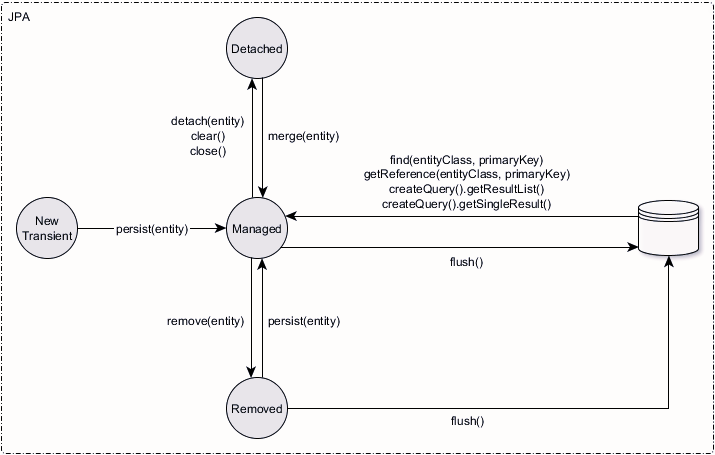
\includegraphics[width=0.75\linewidth]{images/jpaem.png}
        \caption{Possible states for the entities}
    \end{figure}
    According to the previous graph we have that an entity can be in five main states (deleted is omitted in the image): 
    \begin{itemize}
        \item New: the entity is unknown to the entity manager, has no persistent identity, and has no tuple associated. 
        \item Managed: the entity is associated with persistence context, changes to objects automatically, and synchronizes to database. 
        \item Detached: the entity has an identity potentially associated with a database tuple, but changes are not automatically propagated to the database.
        \item Removed: the entity is scheduled for removal from the database.
        \item Deleted: the entity is erased from the database. 
    \end{itemize}

    \subsection{Application architecture}
    In Java Enterprise Edition the client exploits the services the EJB container to connect to the entity manager. In particular, the business level interacts with 
    the entity manager. The advantage of the EJB is that this container provides the support to make JPA entity method calls transactional through the automatic creation 
    of transactions. 
    \begin{figure}[H]
        \centering
        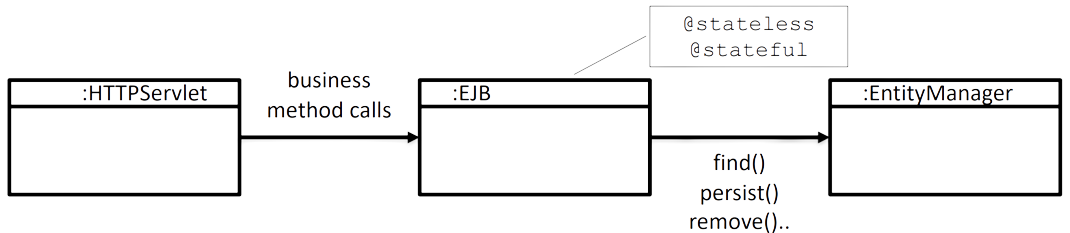
\includegraphics[width=0.75\linewidth]{images/jee1.png}
    \end{figure}
    The transactions exist at three levels: 
    \begin{itemize}
        \item DBMS transactions: they are managed by the DBMS and use SQL. 
        \item Resource-local transactions: they are managed by the application and use the JDBC connection interface. They are mapped to the JDBC. 
        \item Container transaction: they are managed by the application or the container and use the JTA interface. They are mapped to the JDBC. 
    \end{itemize}
    The level used by the entity manager is the container transaction one. After defining a business object, the container injects the entity manager into it. The 
    container manages instances of the entity manager transparently to the application. The container provides the transaction needed for saving the modifications made 
    to the entities of the persistence context associated with the entity manager into the database. 
    \begin{example}
        Definition of a business object EJB: 
        \begin{lstlisting}[style=Java]
@Stateless 
public class myEJBService {
    @PersistenceContext(unitName = "MyPersistenceUnit")
    private EntityManager em; 
}
        \end{lstlisting}
    \end{example}
    When a client calls a method of a business object that exploits a container managed entity manager for persistence, the container provides a transaction for saving 
    the modifications to the database (if the same transaction is called multiple times it will be reused). Note that this is the most common and default behavior, but 
    the business objects methods can be annotated to specify a different way to use the transactions provided by the container. A method can be annotated to obtain the 
    desired transactional behaviour with @TransactionAttribute(TransactionAttributeType.type), where type can be: 
    \begin{itemize}
        \item Mandatory: a transaction is expected to have already been started and be active when the method is called. If no transaction is active, an exception is thrown.
        \item Required: the default, if no transaction is active one is started. If one is active this is used.
        \item Requires$\_$new: the method always needs to be in its own transaction. Any active transaction is suspended. 
        \item Supports: the method does not access transactional resources, but tolerates running inside one if it exists.
        \item Not$\_$supported: the method will cause the container to suspend the current transaction if one is active when the method is called. 
        \item Never: the method will cause the container to throw an exception if a transaction is active when the method is called.
    \end{itemize}

    \section{Benefits of Java Persistence API}
    The main benefits of using the Java Persistence API are: 
    \begin{itemize}
        \item No need to write SQL code.
        \item Application code ignores table names, since the mapping is expressed via annotations with defaults. 
        \item No need to create/destroy the connection. 
        \item No need to create and terminate the transaction. 
        \item Business objects methods are automatically made transactional. 
        \item Default transactional behaviour, with annotations to specify different transaction management policies. 
    \end{itemize}
\end{document}